\section{Illumination globale}

\begin{frame}{Remerciements}
    Cette partie du cours est un extrait de cours de \href{https://maverick.inria.fr/Members/Nicolas.Holzschuch/}{Nicolas Holzschuch}. 
\end{frame}

\begin{frame}{Eclairage direct versus indirect}
    \begin{columns}
        \begin{column}{0.49\textwidth}
            \begin{center}
                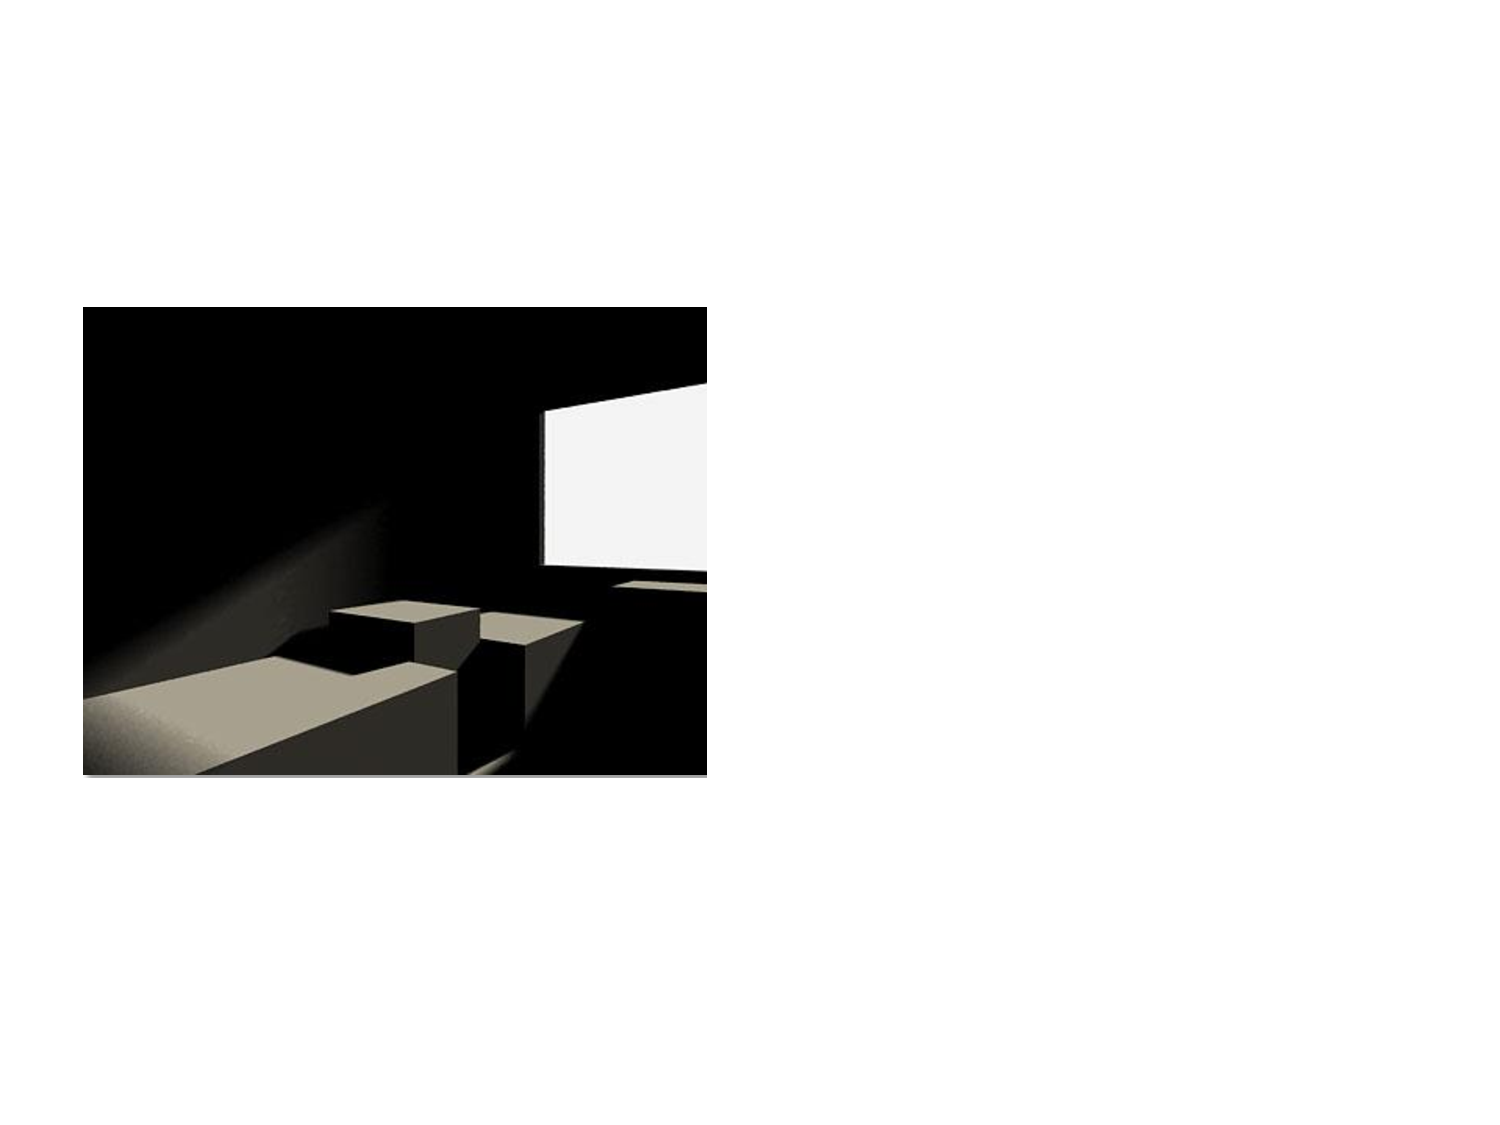
\includegraphics[width=\columnwidth]{figs/eclairage-direct.pdf}
                Eclairage direct : propriétés locales 
            \end{center}
        \end{column}
        \begin{column}{0.49\textwidth}
            \begin{center}
                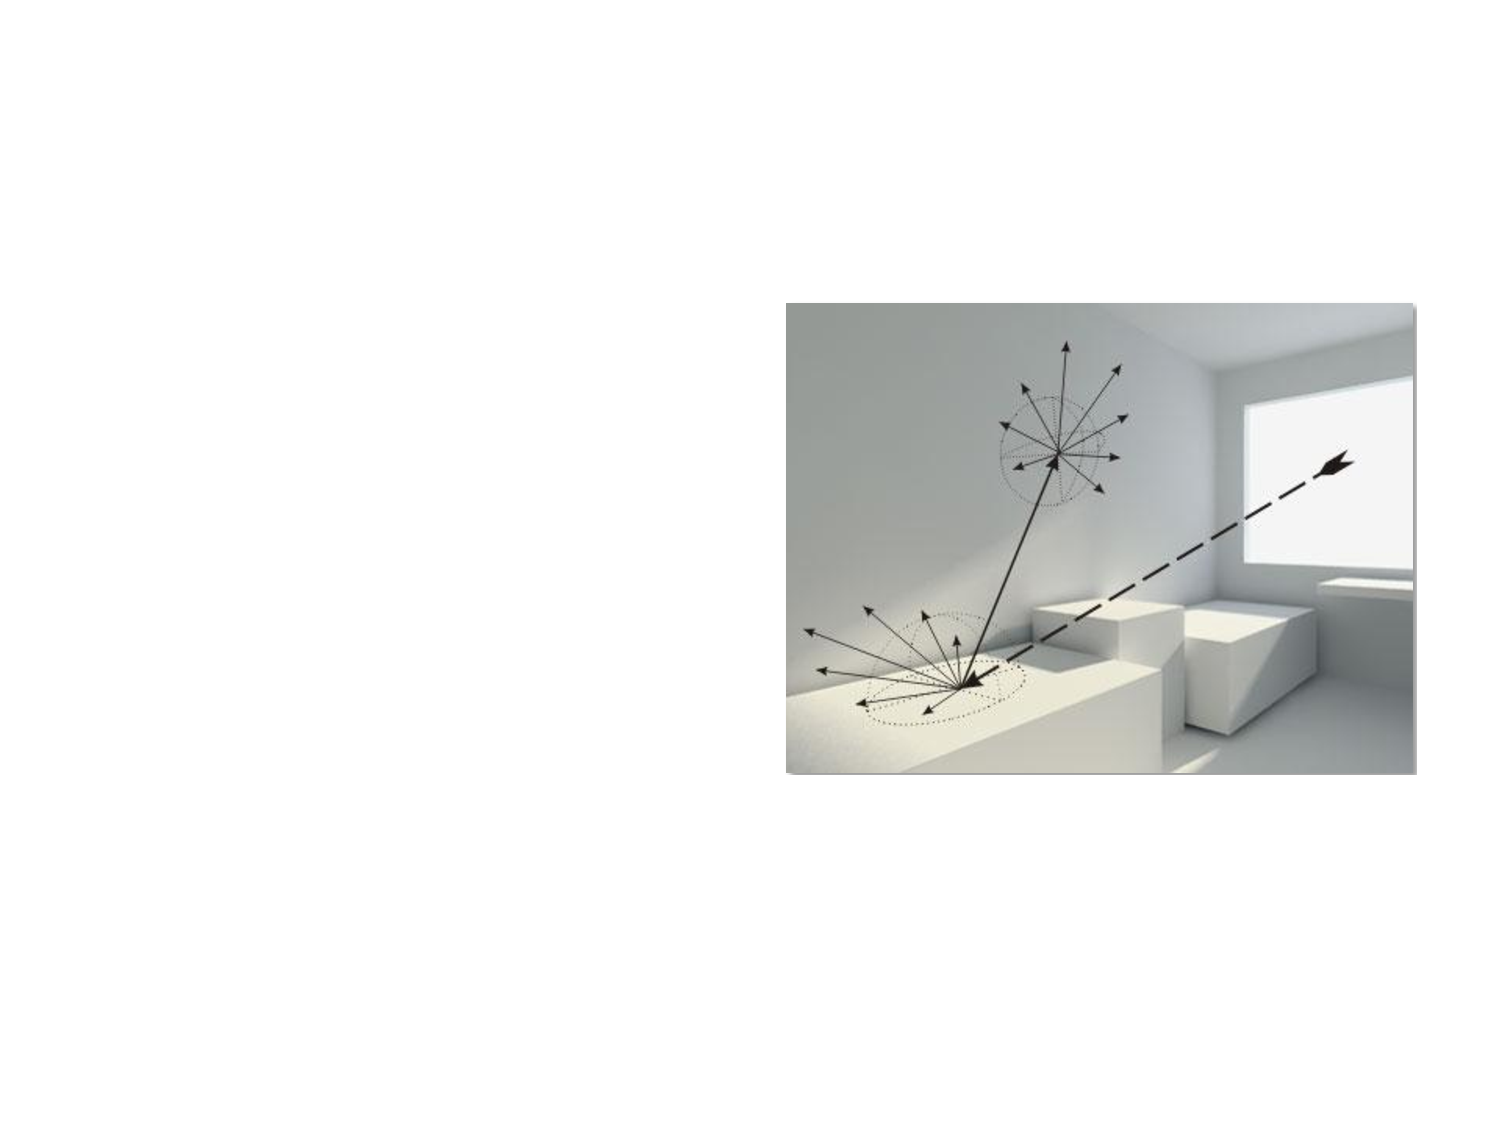
\includegraphics[width=\columnwidth]{figs/eclairage-indirect.pdf}
                Eclairage indirect : problème global
            \end{center}
        \end{column}
    \end{columns}
\end{frame}

\begin{frame}{Eclairage global versus local}
\begin{itemize}
    \item Jusqu'ici des propriétés locales 
    \begin{itemize}
        \item Modèle de Gouraud, de Phong, lissage 
        \item Placage de textures 
    \end{itemize}
    \item Algorithmes locaux
    \begin{itemize}
        \item Z-buffer, Peintre
    \end{itemize}
    \item Très (très) rapide 
\end{itemize}    
\end{frame}

\begin{frame}{Résultat}
    \begin{columns}
        \begin{column}{0.49\textwidth}
            \begin{center}
                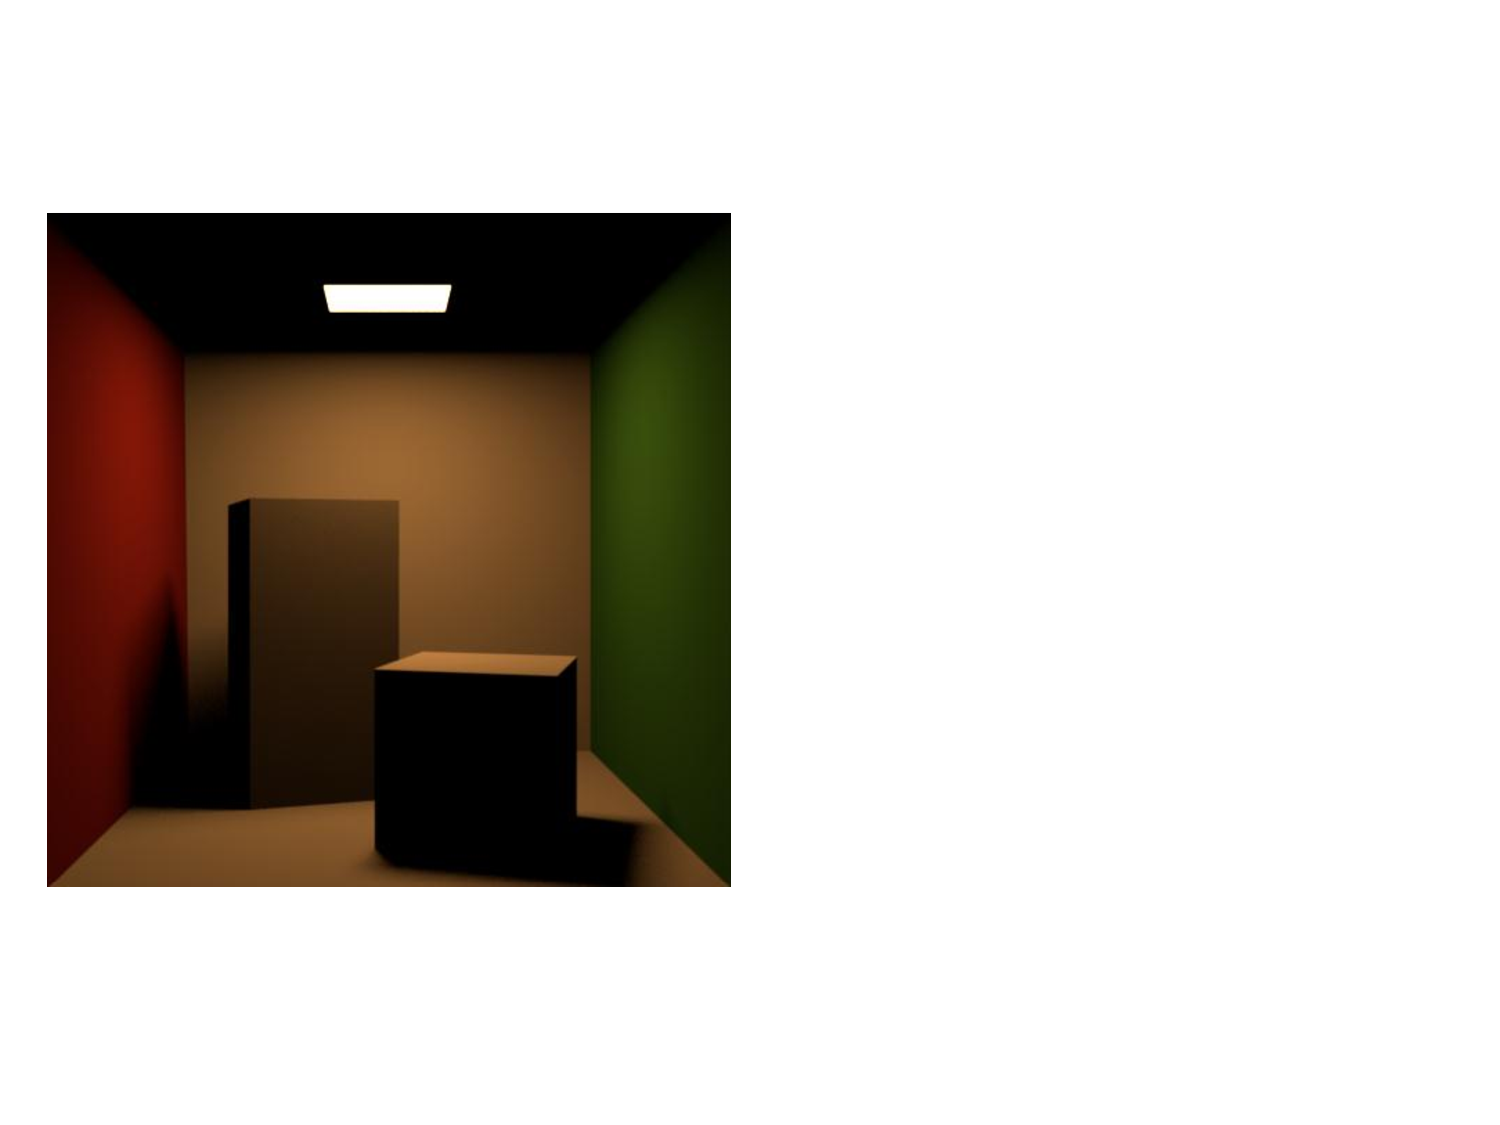
\includegraphics[width=\columnwidth]{figs/rendu-direct.pdf}
                Eclairage direct 
            \end{center}
        \end{column}
        \begin{column}{0.49\textwidth}
            \begin{center}
                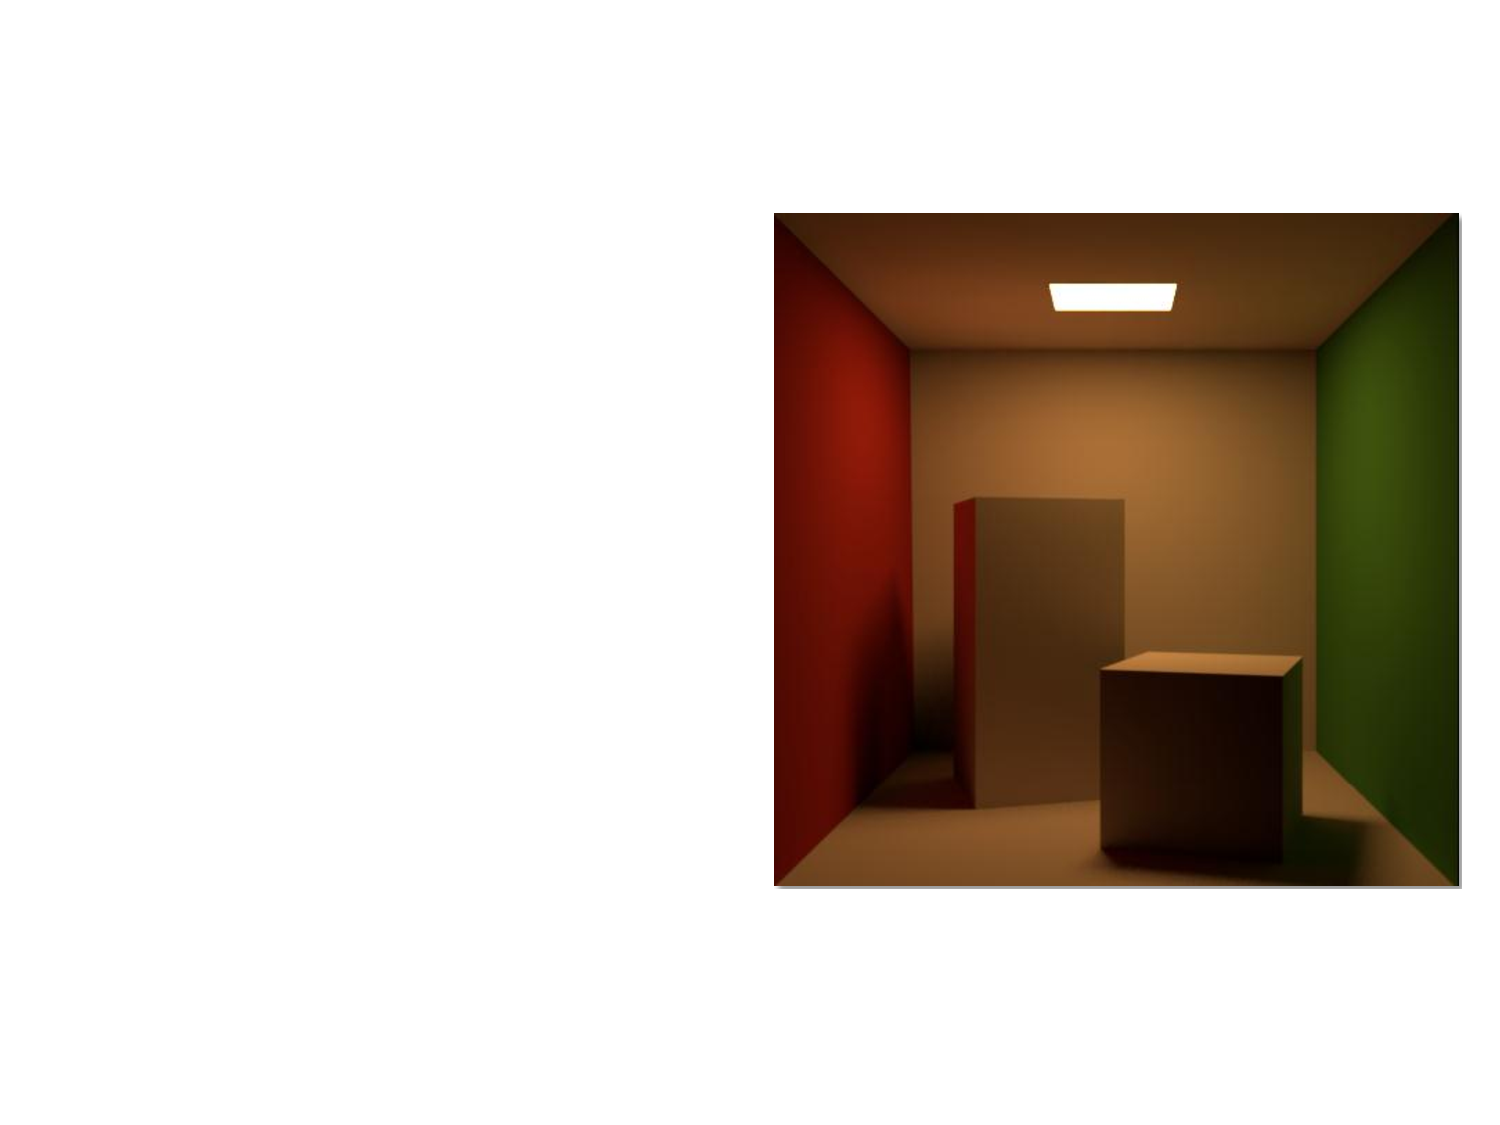
\includegraphics[width=\columnwidth]{figs/rendu-indirect.pdf}
                Eclairage indirect 
            \end{center}
        \end{column}
    \end{columns}
\end{frame}

\begin{frame}{Motivation}
    \begin{center}
        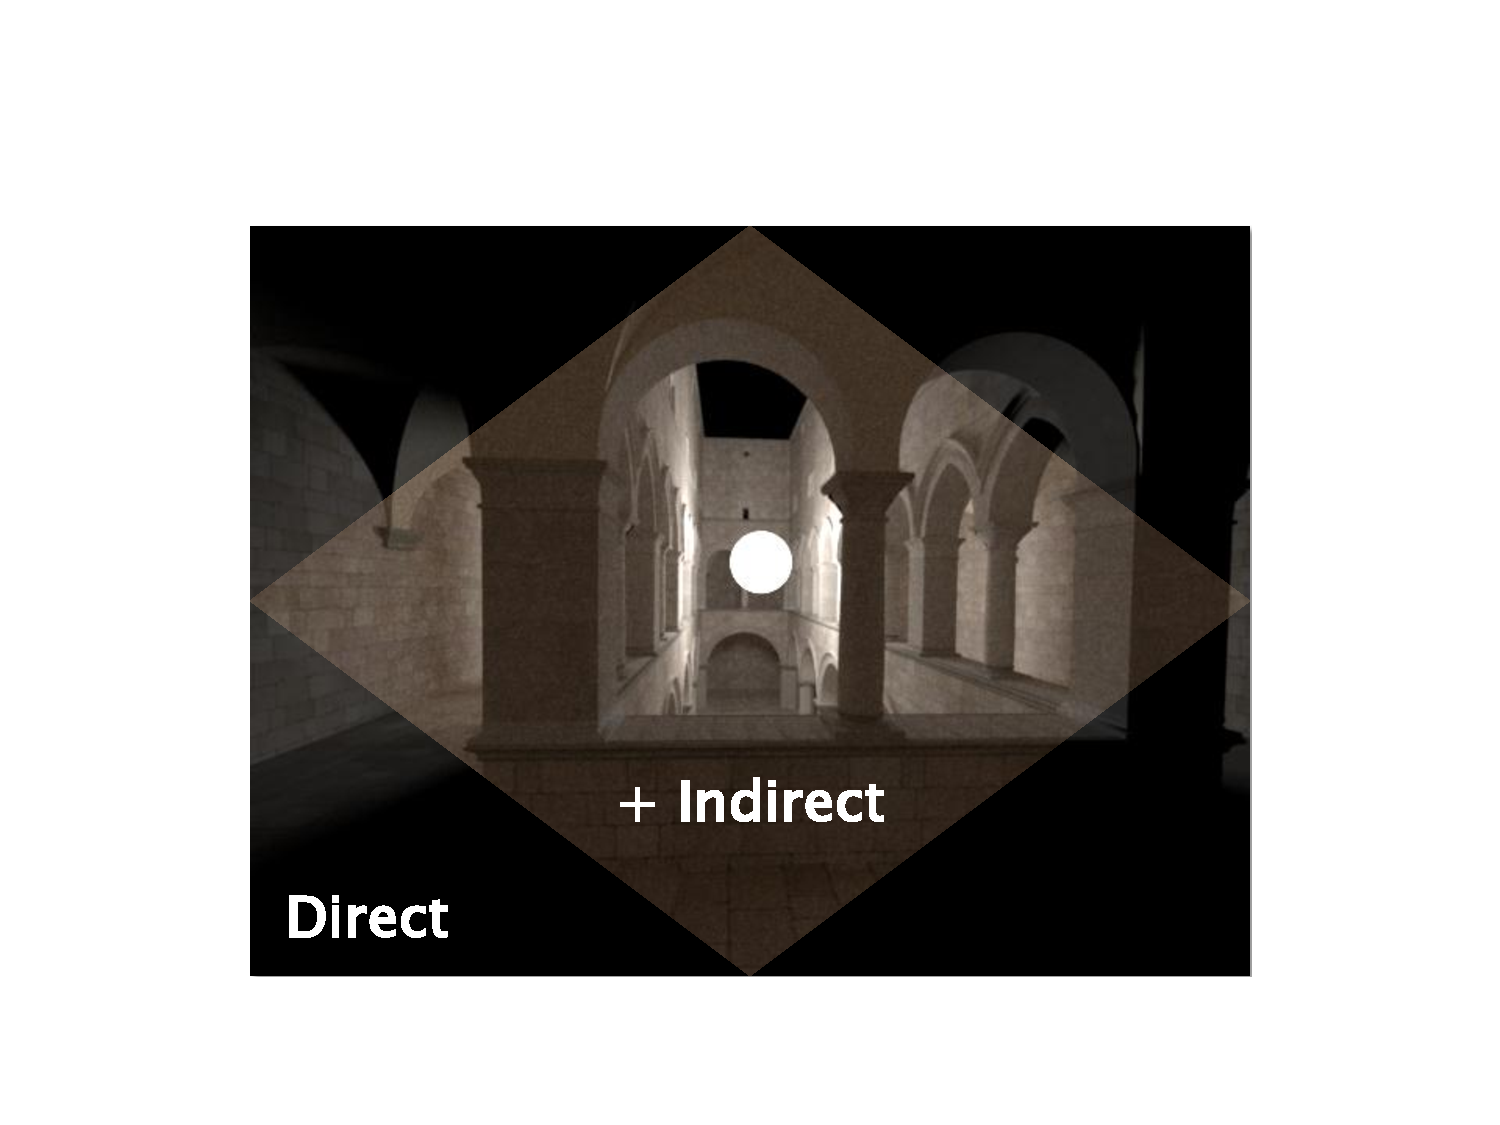
\includegraphics[width=.7\textwidth]{figs/motivation.pdf}
    \end{center}
\end{frame}

\begin{frame}{Illumination globale}
\begin{itemize}
    \item Interactions entre objets 
    \item Transport de la lumière 
    \item Réflexions, réfraction, diffusion
    \item Conservation de l'énergie lumineuse 
\end{itemize}
\begin{center}
    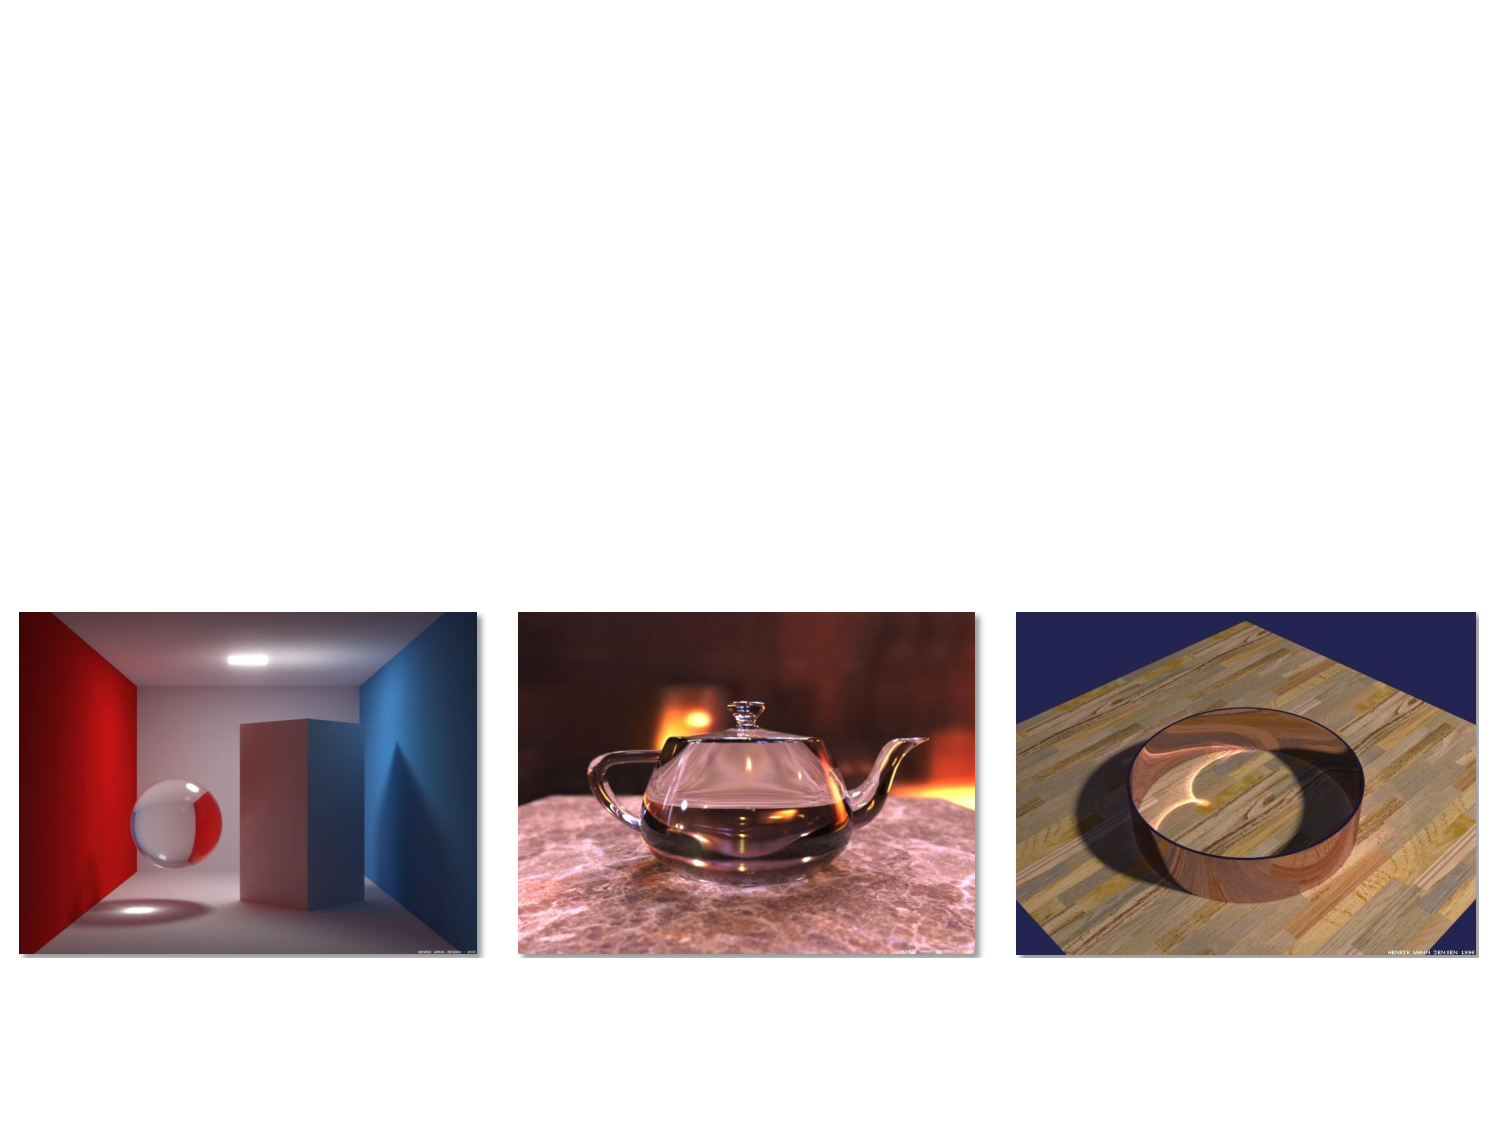
\includegraphics[width=\textwidth]{figs/illumination-globale.pdf}
\end{center}
\end{frame}

\begin{frame}{Equation de l'éclairage}
    \begin{itemize}
        \item Hypothèses 
        \begin{itemize}
            \item Equilibre énergétique 
            \item Conservation de l'énergie ... lumineuse 
            \item i.e. pas d'échanges entre différents types d'énergie 
        \end{itemize}
        \item Energie lumineuse (radiance) en un point (petite unité de surface)
        \item \begin{itemize}
            \item Energie émise (source de lumière)
            \item + énergie réfléchie depuis les autres surfaces
        \end{itemize}
    \end{itemize}
\end{frame}

\begin{frame}{Equation de l'éclairage}
\begin{center}
    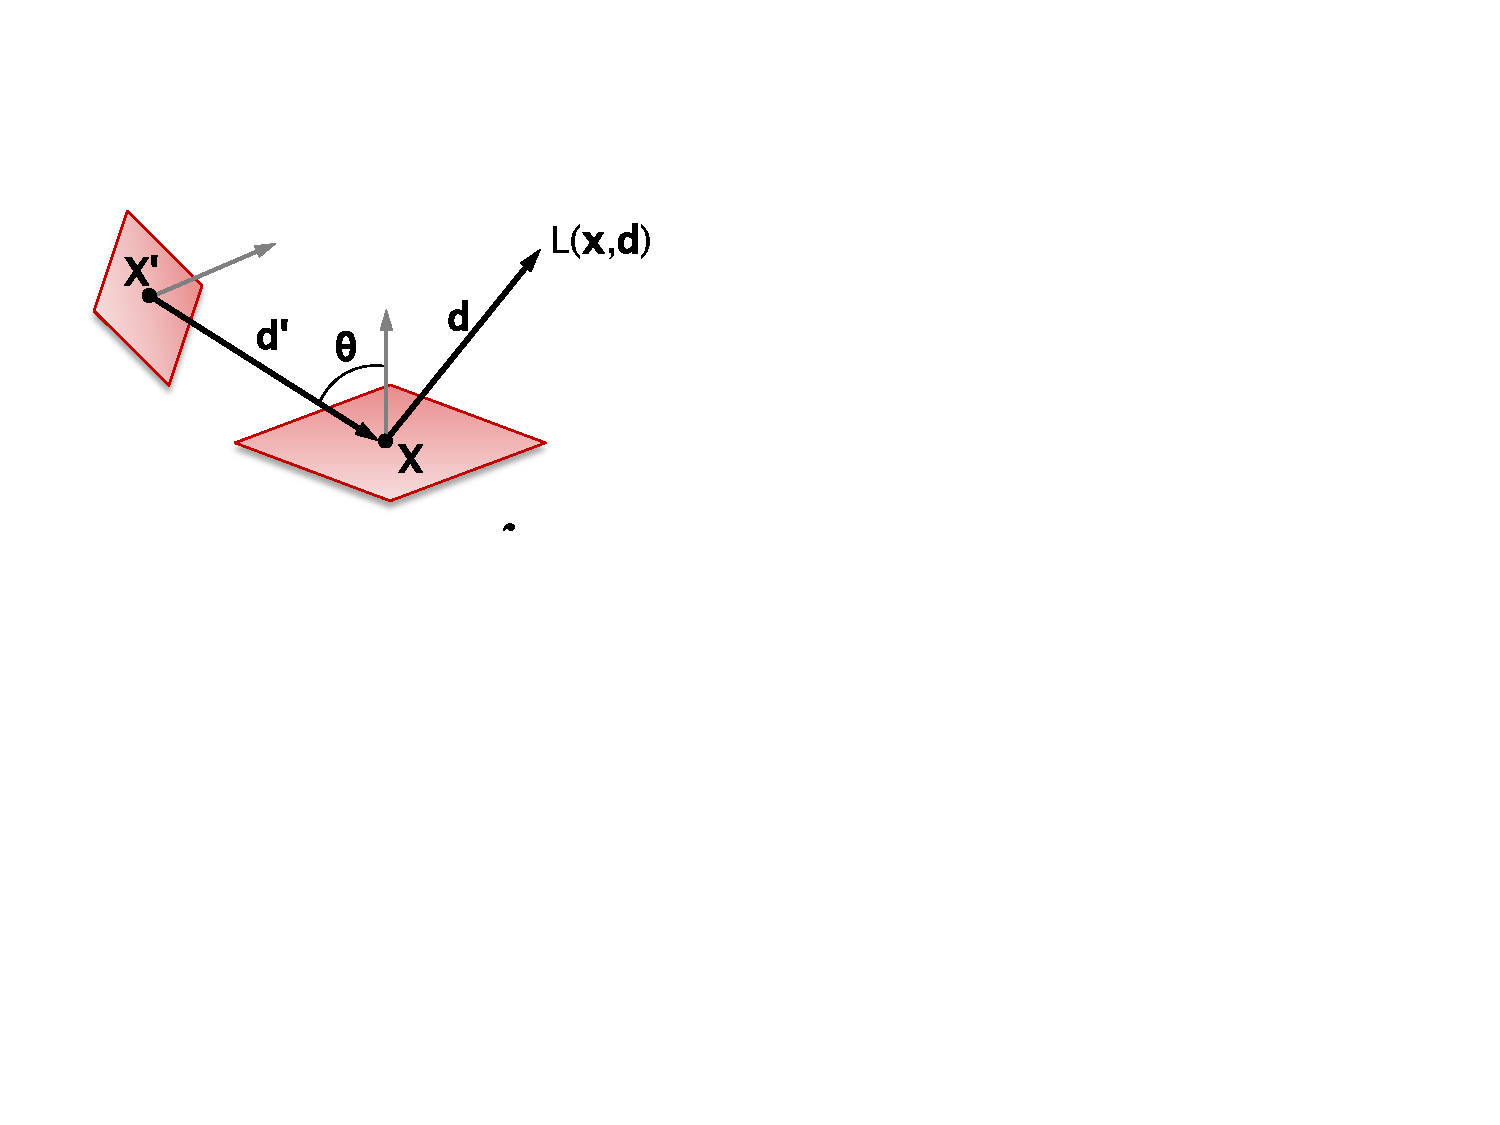
\includegraphics[width=.5\textwidth]{figs/eq-eclairage.pdf}
\end{center}

    $$
    L(x,d) = E(x,d) + \int \rho(x,d,d')v(x,x')L(x',d')G(x,x')  \,\mathrm{d}A 
    $$

\end{frame}


\begin{frame}{Equation de l'éclairage}
    $$
    L(x,d) = E(x,d) + \int \rho(x,d,d')v(x,x')L(x',d')G(x,x')  \,\mathrm{d}A 
    $$
avec :
\begin{itemize}
    \item $L(x,d)$ : radiance sortante en un point $x$ dans la direction $d$ 
    \item $E'x,d)$ : radiance émise par le point $x$, non nulle uniquement pour les sources de lumière
    \item $\int \rho(x,d,d')v(x,x')L(x',d')G(x,x')  \,\mathrm{d}A$ : intégration des contributions de toutes les surfaces, dont
    \begin{itemize}
        \item $L(x',d')$ : radiance incidente depuis $x'$ dans la direction $d'$
        \item $\rho(x,d,d')$ : réflectance (BRDF) de la surface en $x$ 
        \item $v(x,x')$ : visibilité entre $x$ et $x'$ : 0 ou 1 
        \item $G(x,x')$ : description de la relation géométrique entre les deux surfaces en $x$ et $x'$
    \end{itemize}
\end{itemize}
\end{frame}

\begin{frame}{BRDF : Bi-directional Reflectance Distribution Function}
    \begin{columns}
        \begin{column}{0.6\textwidth}
            \begin{itemize}
                \item Rapport entre la radiance dans la direction sortante et le flux de radiance dans la direction entrante 
                \item C'est une distribution 
                \item Unité : sr$^{-1}$
                \item Deux cas particuliers 
                \begin{itemize}
                    \item Réflecteur diffus idéal : distribution uniforme
                    \item Réflecteur spéculaire idéal : distribution de Dirac
                \end{itemize}
                \item En pratique, la BRDF dépend de la longueur d'ondes
            \end{itemize}                 
        \end{column}
        \begin{column}{.39\textwidth}
            \begin{center}
                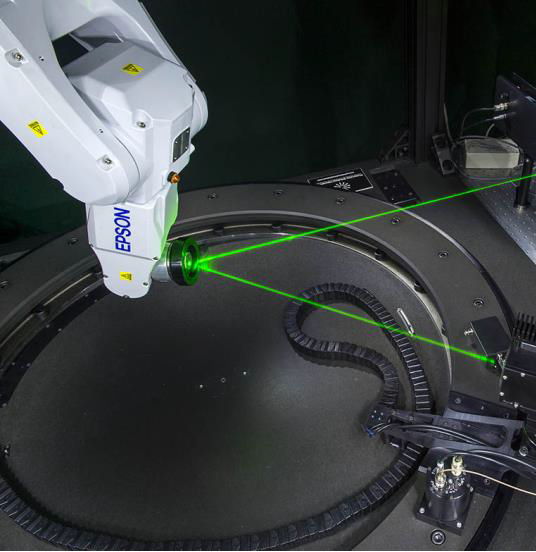
\includegraphics[width=\columnwidth]{figs/BiRT.png}
            \end{center}
        \end{column}
    \end{columns}
 \end{frame}

\begin{frame}{Equation de l'éclairage : solutions}
\begin{block}{Problème}
    Solution analytique générale impossible !
\end{block}
\begin{itemize}
    \item 2 grandes familles de solutions approchées
    \item Version (très) simplifiée : l'énergie lumineuse réémise par une facette est proportionnelle  à
    \begin{itemize}
        \item l'énergie reçue par les sources de lumière 
        \item \textcolor{blue}{l'énergie reçue par d'autres facettes : prise en compte des inter-réflexions}
    \end{itemize}
    \item Radiosité 
    \begin{itemize}
        \item tous les objets sont diffus 
    \end{itemize}
    \item Lancer de rayons 
    \begin{itemize}
        \item tous les objets sont spéculaires 
    \end{itemize}
\end{itemize}
\end{frame}

\subsection{Lancer de rayons}

\begin{frame}{Le lancer de rayons}
    \begin{center}
        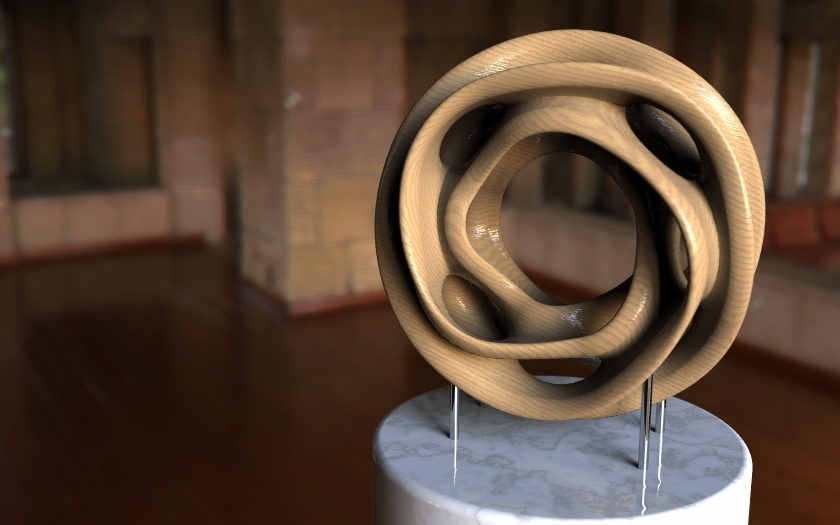
\includegraphics[width=.4\textwidth]{figs/sherk-collins.jpg}\\
        {\tiny "Scherk-Collins sculpture" by Trevor G. Quayle (2008)}
    \end{center}
    \begin{itemize}
        \item Algorithme : Appel, 1968 
        \item Logiciel : Goldstein et Nagel, 1971
        \item Exemple célèbre (et gratuit) : povray, \url{http://www.povray.org}
        \item Idée générale
        \begin{itemize}
            \item Chaque facette est un réflecteur parfait 
            \item Inverser la circulation des rayons lumineux : de l'écran vers les sources de lumière
        \end{itemize}
    \end{itemize}
\end{frame}

\begin{frame}{Inverser le chemin des rayons lumineux}
    \begin{center}
        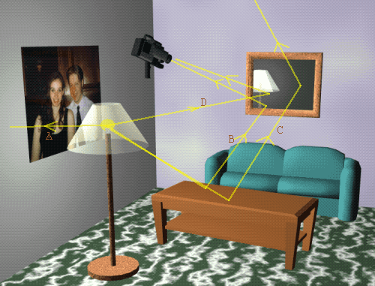
\includegraphics[width=.6\textwidth]{figs/rt-inverse.png}
    \end{center}
    Pourquoi ? 
    L'écran a un nombre fini de pixels, on va lancer un rayon de chaque pixel
\end{frame}

\begin{frame}{Principe}
    \begin{columns}
        \begin{column}{.49\textwidth}
            \begin{itemize}
                \item Pour chaque pixel, on calcule la demi-droite ayant pour origine un pixel du plan image de la caméra et passant par son centre optique 
                \item On cherche ensuite l'intersection entre cette demi-droite et un élément de la scène puis on utilise un modèle d'illumination local
                \item S'il n'y en a pas, le point sera noir
            \end{itemize}
        \end{column}

        \begin{column}{.49\textwidth}
            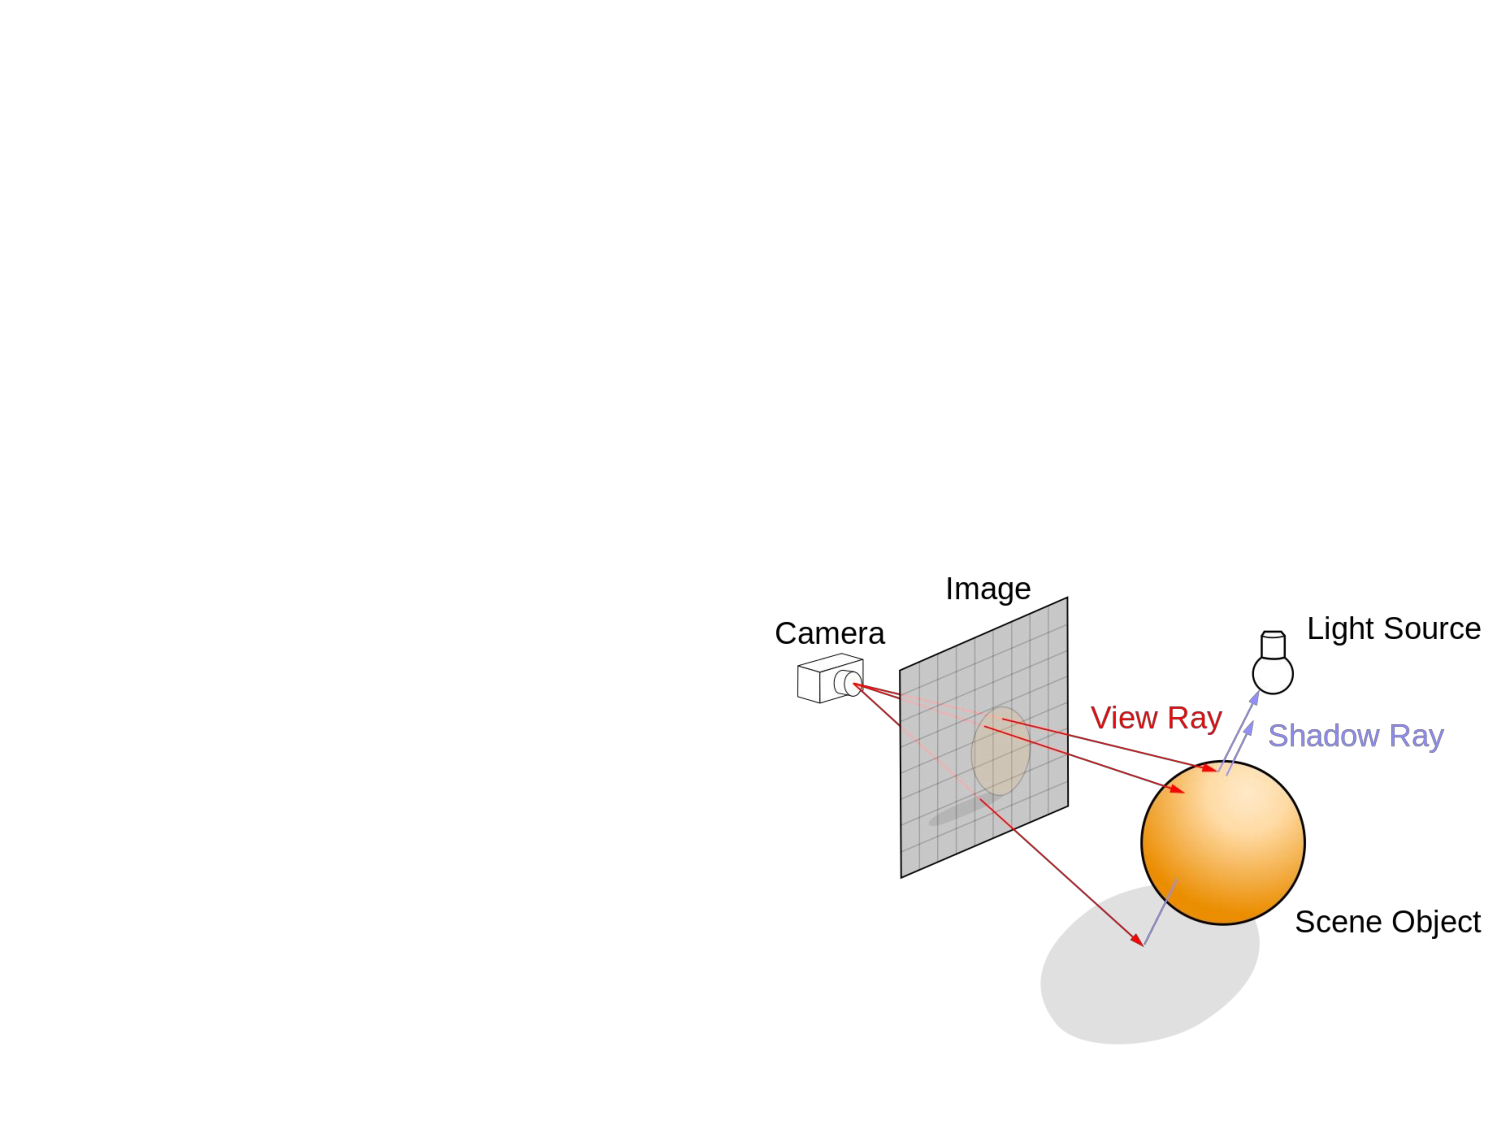
\includegraphics[width=\columnwidth]{figs/raycasting.pdf}
        \end{column}
    \end{columns}
\end{frame}

\begin{frame}{Lancer de rayons selon Whitted}
    \begin{itemize}
        \item Whitted a proposé d'ajouter à cela les lois de la diffraction / réfraction et les réflexions à chaque fois qu'un rayon rencontre un objet de la scène
        \item Cela donne un algorithme récursif : un rayon qui rencontre un objet génère deux autres rayons
        \begin{itemize}
            \item Un rayon réfléchi 
            \item Un rayon transmis
        \end{itemize}
    \end{itemize}
\end{frame}

\begin{frame}{Réflexion}
    \begin{center}
        \animategraphics[loop,controls,width=.5\linewidth]{10}{figs/rt-reflection/}{0}{8}
    \end{center}
\end{frame}

\begin{frame}{Réfraction}
    \begin{center}
        \animategraphics[loop,controls,width=.5\linewidth]{10}{figs/rt-refraction/}{0}{8}
    \end{center}
\end{frame}

\begin{frame}{Loi de Snell-Descartes}
    \begin{center}
        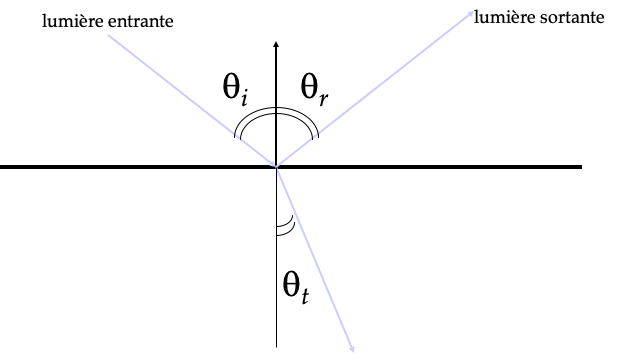
\includegraphics[width=.5\textwidth]{figs/descartes.png}
        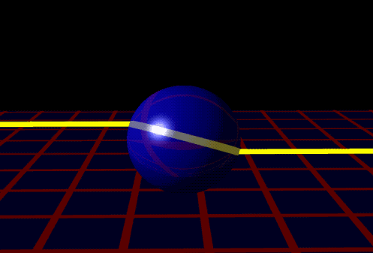
\includegraphics[width=.4\textwidth]{figs/descartes-2.png}
    \end{center}
    $$
        n_i \sin \theta_i = n_t \sin \theta_t
    $$
\end{frame}

\begin{frame}{Jusqu'où ?}
    \begin{center}
        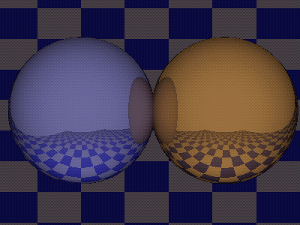
\includegraphics[width=.3\textwidth]{figs/recur-1.png}
        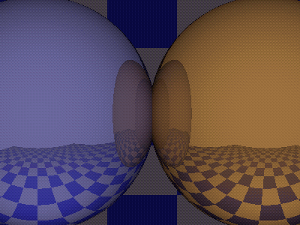
\includegraphics[width=.3\textwidth]{figs/recur-2.png}
        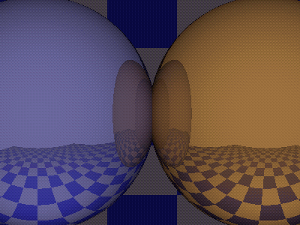
\includegraphics[width=.3\textwidth]{figs/recur-3.png}
    \end{center}
    Complexité exponentielle
\end{frame}

\begin{frame}{Algorithme du lancer de rayons 1/2}
    \begin{algorithmic}[1]
        \For{$u \in [0,...,w]$}
            \For{$v \in [0,...,h]$}
                \State ray = calculateRay(u,v,cam\_params)
                \State color[u][v] = ray\_trace(ray,0)
            \EndFor
        \EndFor
     \end{algorithmic}
\end{frame}

\begin{frame}{Algorithme du lancer de rayons 2/2}
            \begin{algorithmic}[1]
      \Function{ray\_trace}{$r$ : Ray,$depth$ : int}
                \If{depth > MAX\_DEPTH} 
                    \State return background\_color 
                \EndIf
                \State hits = findClosestIntersection(r)
                \If{hits == 0} 
                    \State return background\_color 
                \EndIf
                \State $c_l$ = calculateLocalColor($r$)
                \State refl = calculateReflection($r$)
                \State $c_r$ = raytrace(refl,depth+1)
                \State tran = calculateRefraction($r$)
                \State $c_t$ = raytrace(tran,depth+1)
                \State return $c_l + c_r + c_t$
       \EndFunction 
             \end{algorithmic}
\end{frame}

\begin{frame}{Avantages}
    \begin{itemize}
        \item Elimination des parties cachées incluses dans l'algorithme 
        \item Ombres portées incluses 
        \begin{itemize}
            \item correctes du point de vue géométriques 
        \end{itemize}
        \item Réflexions entre les objets 
        \item Qualité d'image 
        \item Quelques effets possibles 
        \begin{itemize}
            \item Milieux participants (fumée, brouillard)
            \item Mirages 
            \item Bleu atmosphérique 
            \item Effets photographiques (profondeur de champ, déformations de l'objectif)
        \end{itemize}
    \end{itemize}
    
\end{frame}

\begin{frame}{Inconvénients}
    \begin{itemize}
        \item \textbf{Le temps de calcul !}
        \begin{itemize}
            \item les intersections entre primitives sont les opérations les plus fréquentes
        \end{itemize}
        \item L'aliassage 
        \item Le bilan énergétique incorrect 
    \end{itemize}
\end{frame}

\begin{frame}{Accélération du lancer de rayons}
    \begin{itemize}
        \item L'algorithme est massivement parallélisable : le calcul de la couleur des  pixels de l'image sont indépendants les uns des autres 
        \item Les calculs d'intersection peuvent être largement optimisés 
        \begin{itemize}
            \item Boites englobantes 
            \item Partitionnement de l'espace 
        \end{itemize}
    \end{itemize}
\end{frame}

\begin{frame}{Volumes englobants}
    \begin{itemize}
        \item Boite englobantes : parallépipède rectangle (aligné sur les axes ou non)
        \item On teste l'intersection avec la BE avant de tester l'intersection avec l'objet 
        \begin{itemize}
            \item Un test rapide peut en économiser un plus long
        \end{itemize}
        \item On peut utiliser d'autres formes de boites englobantes (sphères notamment) tant que les calculs d'intersection avec une demi-droite sont faciles 
        \item Les boites englobantes peuvent être utilisées aussi de façon hiérarchiques
        \begin{itemize}
            \item Test récursif d'intersection à partir de la BE \emph{racine}
        \end{itemize}
    \end{itemize}
\end{frame}

\begin{frame}{Illustrations}
    \begin{center}
        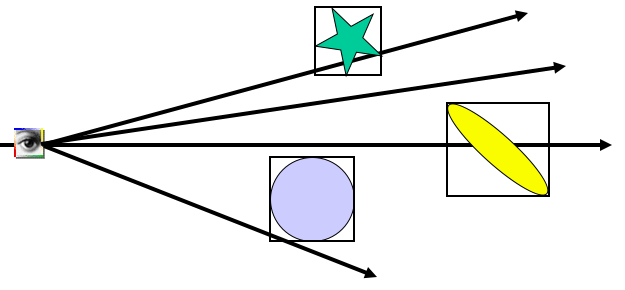
\includegraphics[width=.49\textwidth]{figs/bb-1.png}
        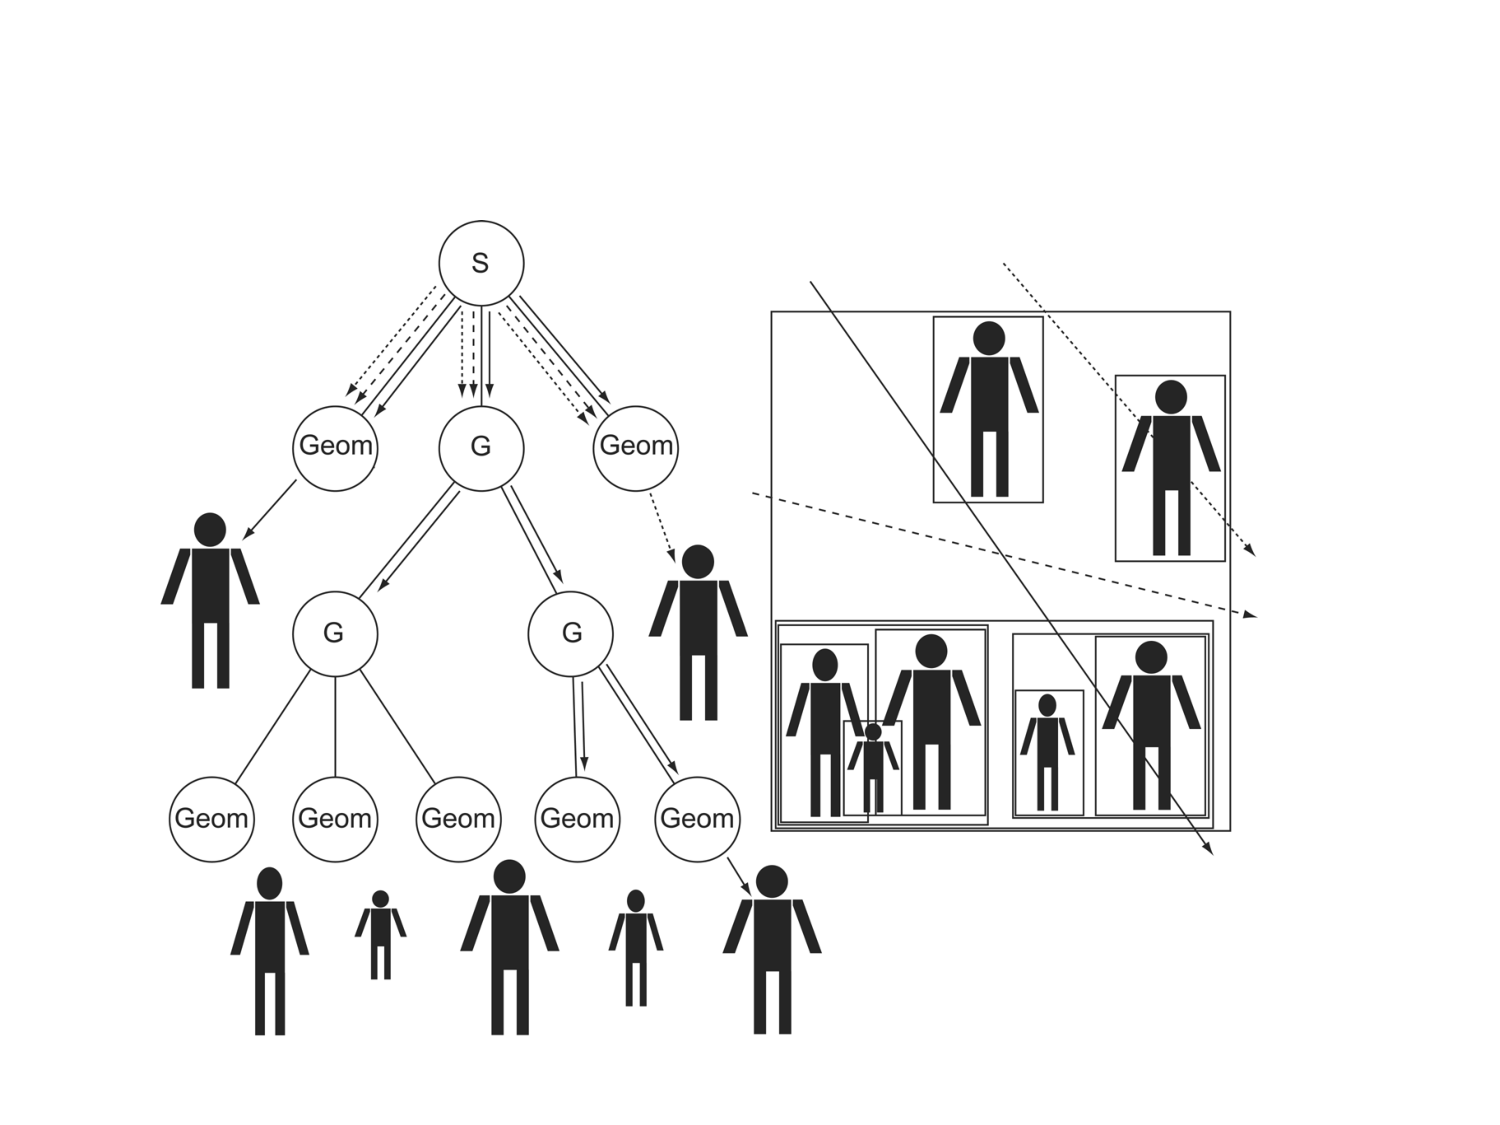
\includegraphics[width=.49\textwidth]{figs/bb-2.pdf}
    \end{center}
\end{frame}

\begin{frame}{Partitionnement de l'espace}
    \begin{itemize}
        \item Grille uniforme 
        \begin{itemize}
            \item Construction d'une grille 3D 
            \item Les objets sont placés dans les cellules de la grille qu'ils touchent 
            \item Intersection rayon avec chacun des objets de chacune des cellules traversées 
        \end{itemize}
        \item Organisation hiérarchique de grilles 
        \begin{itemize}
            \item kd-tree, octree, bsp-tree
        \end{itemize} 
    \end{itemize}
    \begin{center}
        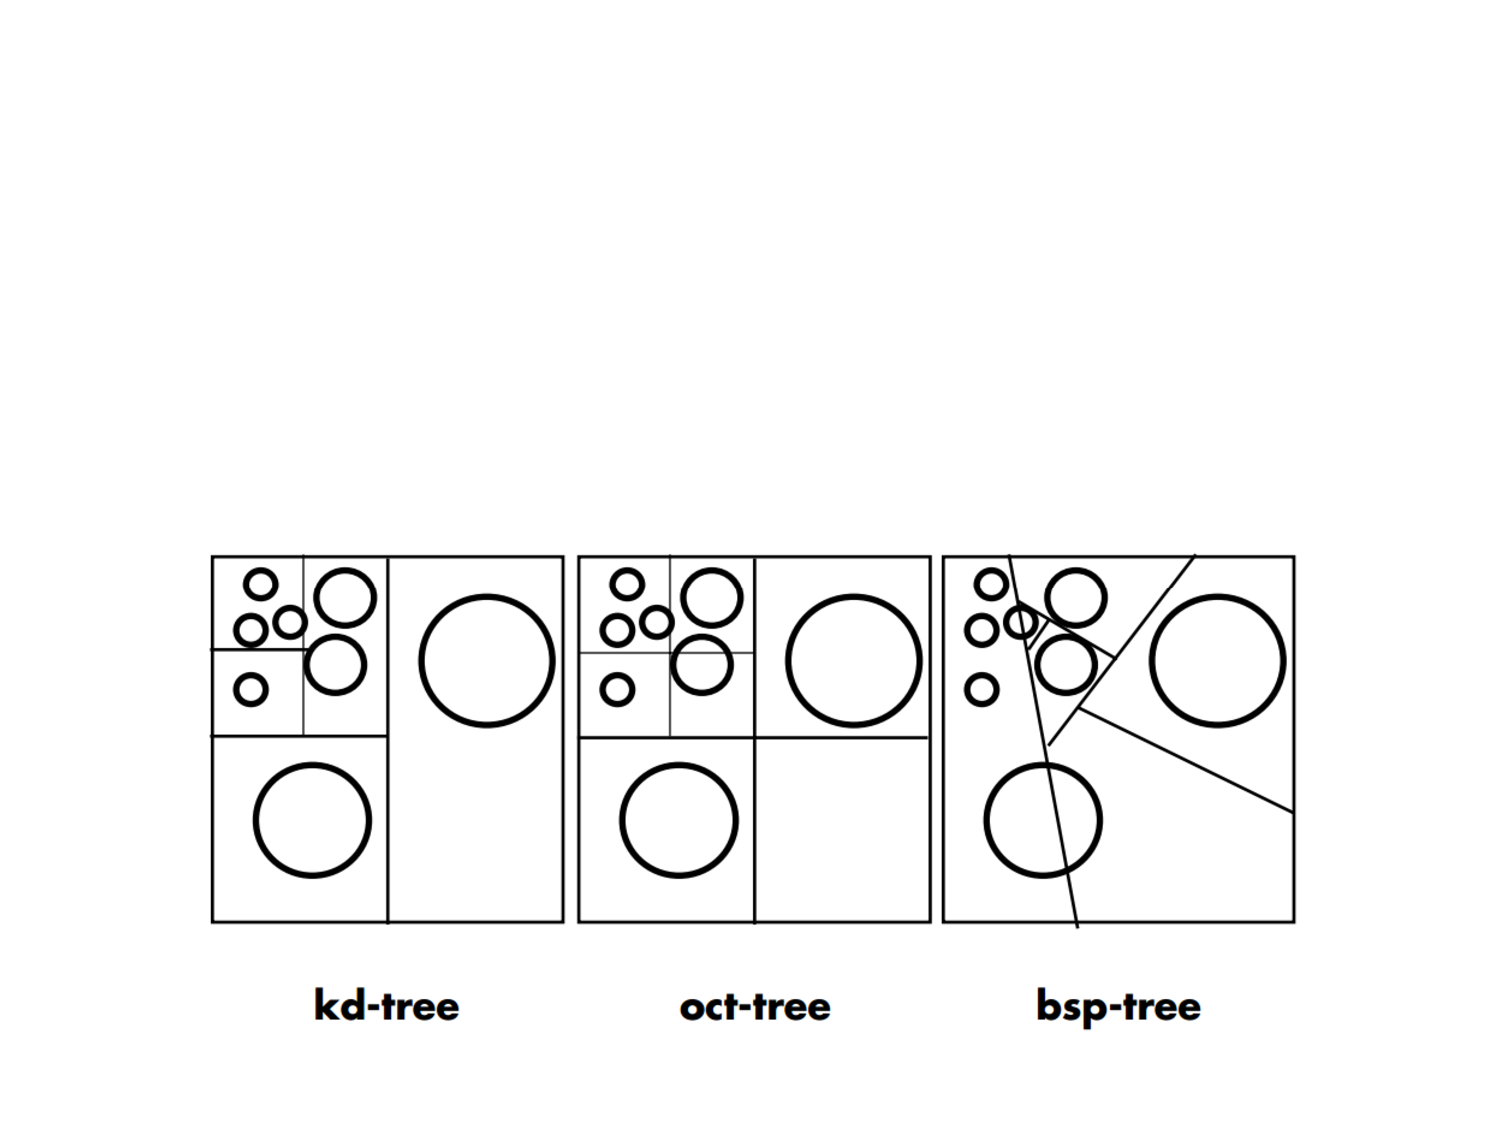
\includegraphics[width=.8\textwidth]{figs/trees.pdf}
    \end{center}
\end{frame}

\begin{frame}{Comparatif}
    \begin{itemize}
        \item Hiérarchie de boîtes englobantes 
        \begin{itemize}
            \item construction longue, requêtes rapides 
        \end{itemize}
        \item Grille uniforme 
        \begin{itemize}
            \item construction rapide, requêtes rapides ... si on est à la bonne résolution
        \end{itemize}
        \item Octrees, BSP-trees
        \begin{itemize}
            \item très simple, construction rapide, requêtes plus longues
        \end{itemize}
    \end{itemize}
\end{frame}

\subsection{Méthodes de radiosité}

\begin{frame}{Méthodes de radiosité}
    \begin{itemize}
        \item Idées 
        \begin{itemize}
            \item Matériaux purement diffus 
            \item Prendre en compte \textbf{toutes} les inter-réflexions
        \end{itemize}
        \item Radiance et BRDF sont indépendantes de la direction
        \item Simplification de l'équation de l'éclairage 
    \end{itemize} 
\end{frame}


\begin{frame}{L'équation de la radiosité}
    \begin{itemize}
        \item C'est une discrétisation de l'équation de l'éclairage, indépendante du point de vue
        \item Environnement échantillonné sous la forme de petits éléments de surfaces (les \emph{patches}), de taille finie, émettant et réfléchissant la lumière de façon uniforme sur leur surface 
    \end{itemize}
    \begin{center}
    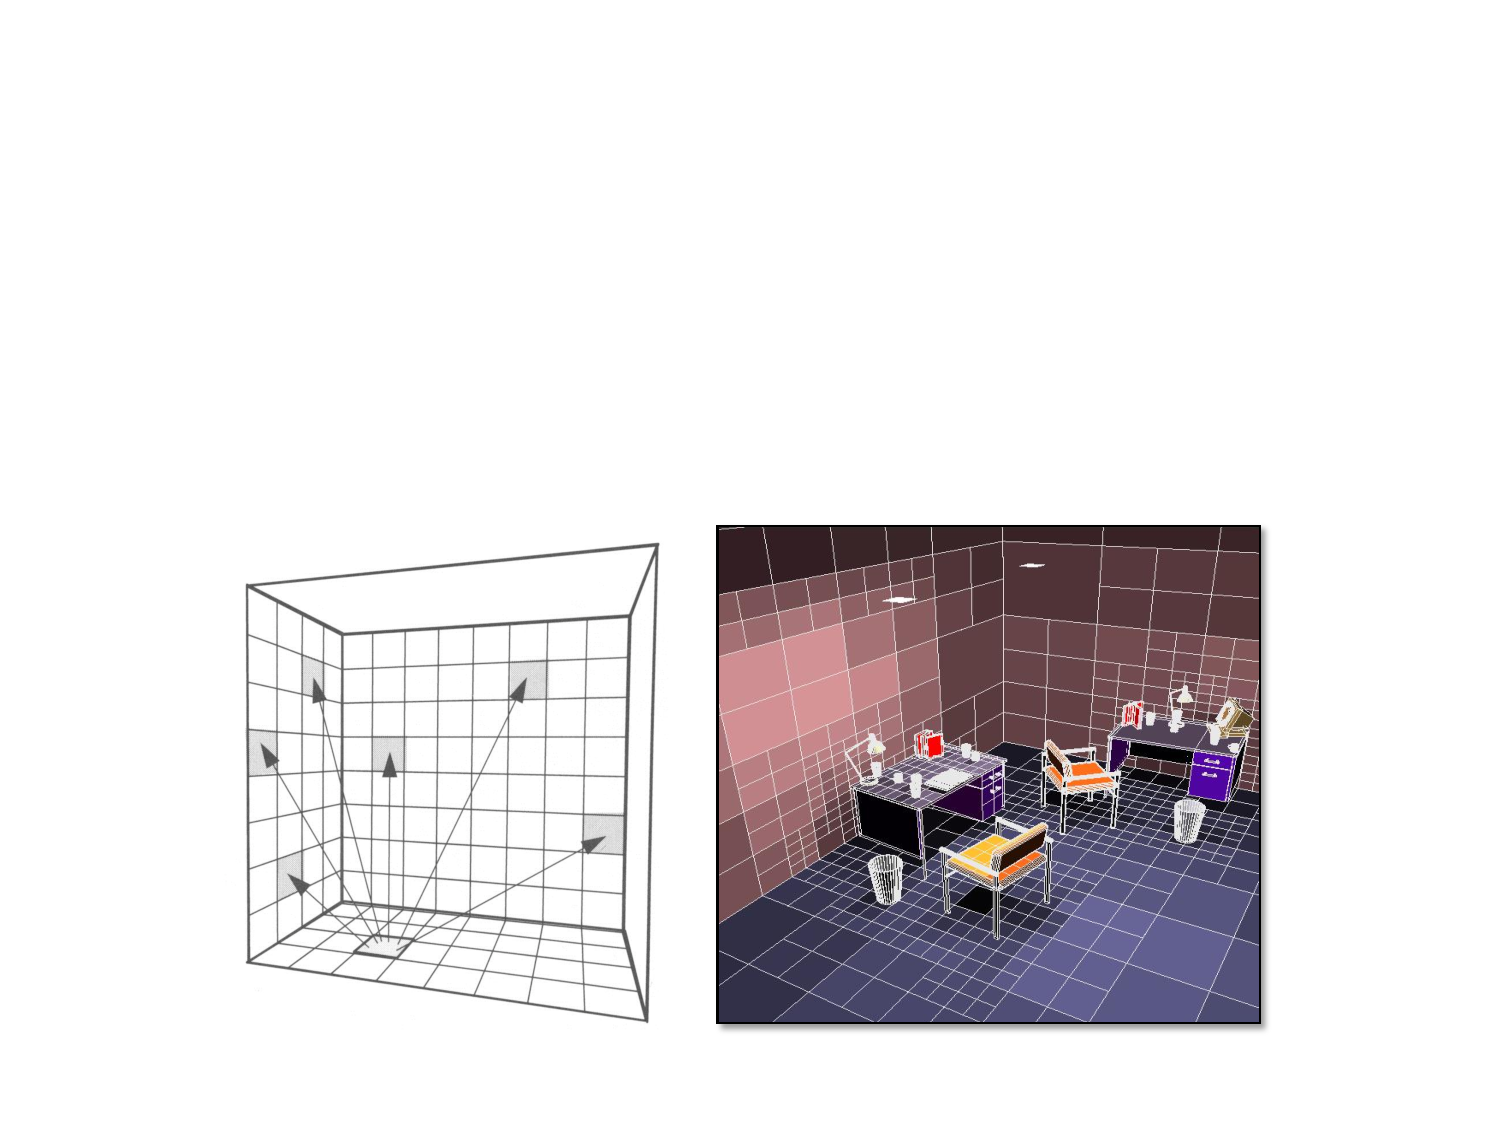
\includegraphics[width=0.6\textwidth]{figs/patches.pdf}
    \end{center}
\end{frame}

\begin{frame}{Simplification et discrétisation}
    $$
    L(x,d) = E(x,d) + \int \rho(x,d,d')v(x,x')L(x',d')G(x,x')  \,\mathrm{d}A 
    $$

    \begin{itemize}
        \item Forme simplifiée 
    \end{itemize}

    $$
    B(x) = E(x) + \rho_x \int B(x') v(x,x') G(x,x') \,\mathrm{d}A 
    $$

    \begin{itemize}
        \item $v(x,x') G(x,x')$ : facteur de forme 
        \item Discrétisation 
    \end{itemize}

    $$
    B_i = E_i + \rho_i \Sigma_j F_{ji} B_j A_j/A_i
    $$

\end{frame}

\begin{frame}{Equation de la radiosité}
    $$
    B_i = E_i + \rho_i \Sigma_j F_{ji} B_j A_j/A_i
    $$

    \begin{itemize}
        \item $B_i$ : radiosité (constante) du i-ème élément de surface
        \item $E_i$ : puissance lumineuse émise par le i-ème élément de surface
        \item $A_i$ : aire du patch $i$
        \item $F_{ji}$ = facteur de forme qui caractérise la proportion d'énergie quittant le patch $j$ qui arrive sur le patch $i$
    \end{itemize}
\end{frame}

\begin{frame}{Version matricielle}
    $$
    \begin{pmatrix}
        B_0 \\ \\ B_n
    \end{pmatrix}
    = 
    \begin{pmatrix}
        E_0 \\ \\ E_n
    \end{pmatrix}
    +
    \begin{pmatrix}
        \rho_i F_{ji}       
    \end{pmatrix}
    \begin{pmatrix}
        B_0 \\ \\ B_n
    \end{pmatrix}
    \Longleftrightarrow
    \boldsymbol{B} = \boldsymbol{E} + \boldsymbol{MB}
$$
\begin{itemize}
    \item Système linéaire matriciel 
    \item Résolution itérative (par longueur d'onde)
    \item Stockage de l'équation : un problème en soi 
\end{itemize}
\end{frame}

\begin{frame}{Facteurs de forme}

    \begin{columns}
        \begin{column}{.4\textwidth}
            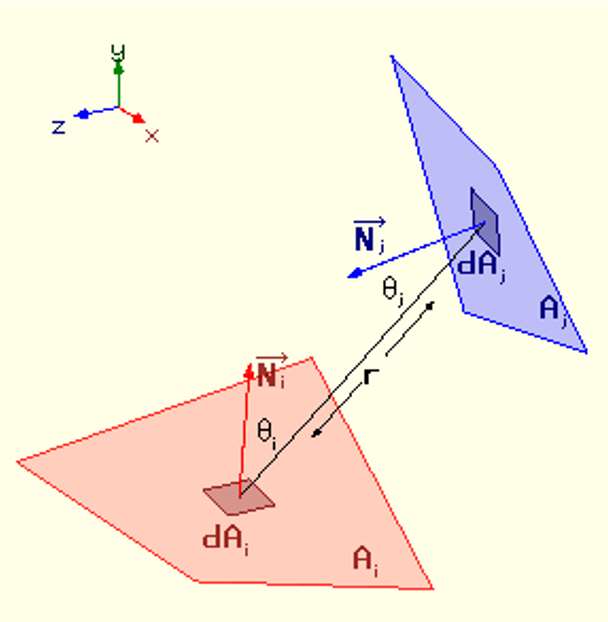
\includegraphics[width=\columnwidth]{figs/ff.png}
        \end{column}
        \begin{column}{.6\textwidth}
            $$
            F_{ij} = \int_{A_i} \int_{A_j} v(x,x') \frac{\cos \theta \cos \theta'}{\pi r^2} dx dx'
        $$
        
        \begin{itemize}
            \item Problème : pas de solution analytique 
            \item Solution : projection sur une hémisphère ou un hémicube 
        \end{itemize}
                    
        \end{column}
    \end{columns}
\end{frame}

\begin{frame}{Pipeline}
    \begin{center}
        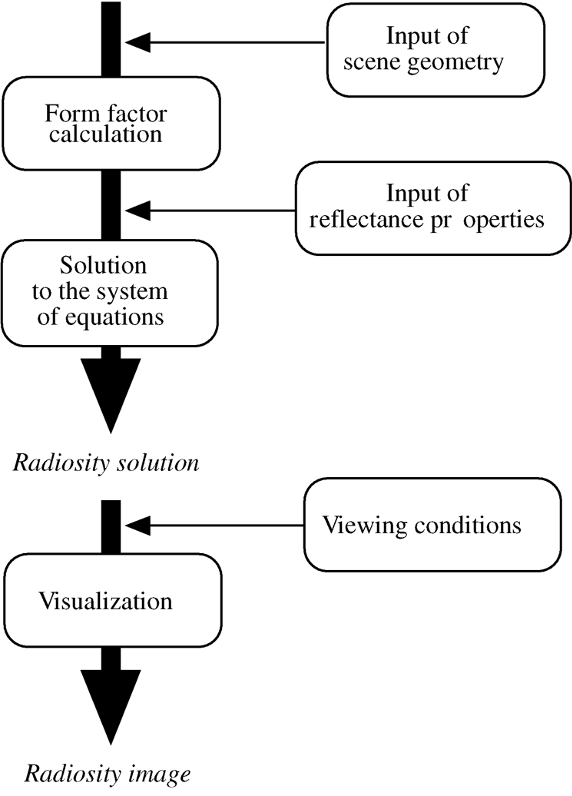
\includegraphics[width=.4\textwidth]{figs/radiosity-pipeline.png}
    \end{center}
\end{frame}

\begin{frame}{Intérêt}
    \begin{center}
        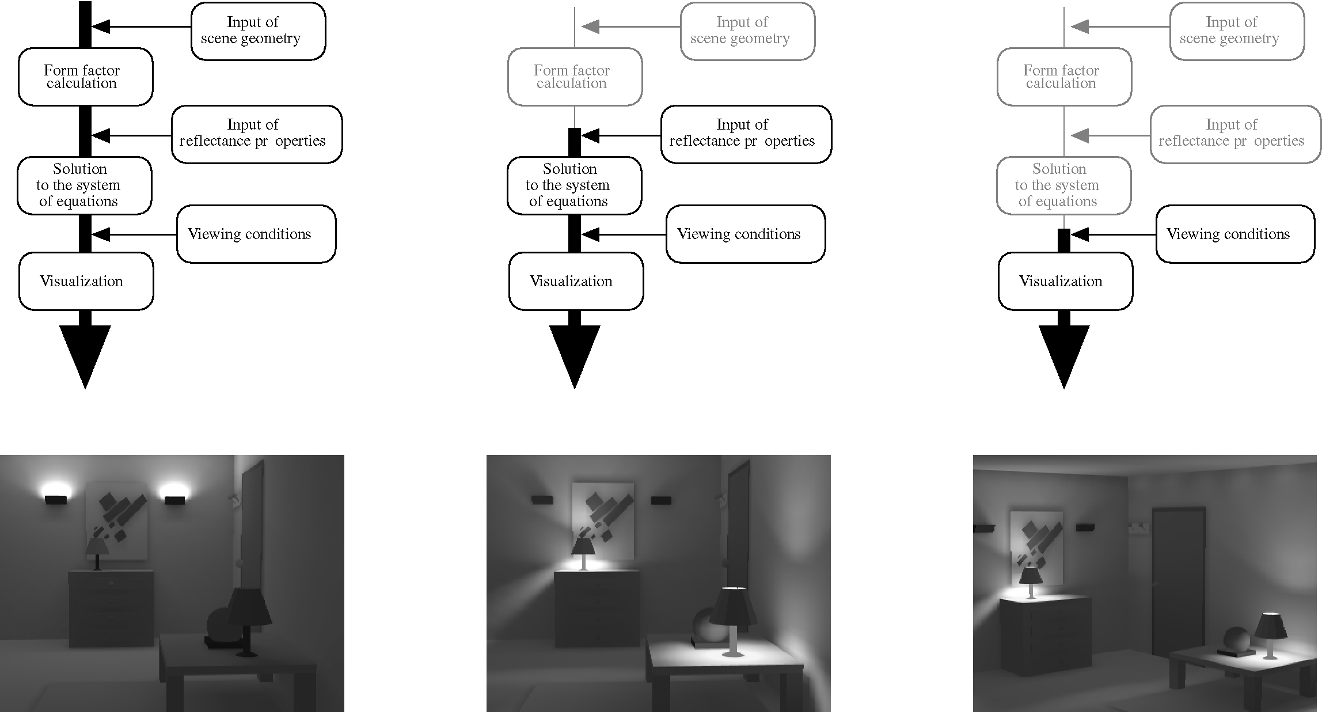
\includegraphics[width=\textwidth]{figs/radiosity-pipeline-2.png}
    \end{center}
\end{frame}

\begin{frame}{Résolution itérative illustrée}
    \begin{center}
        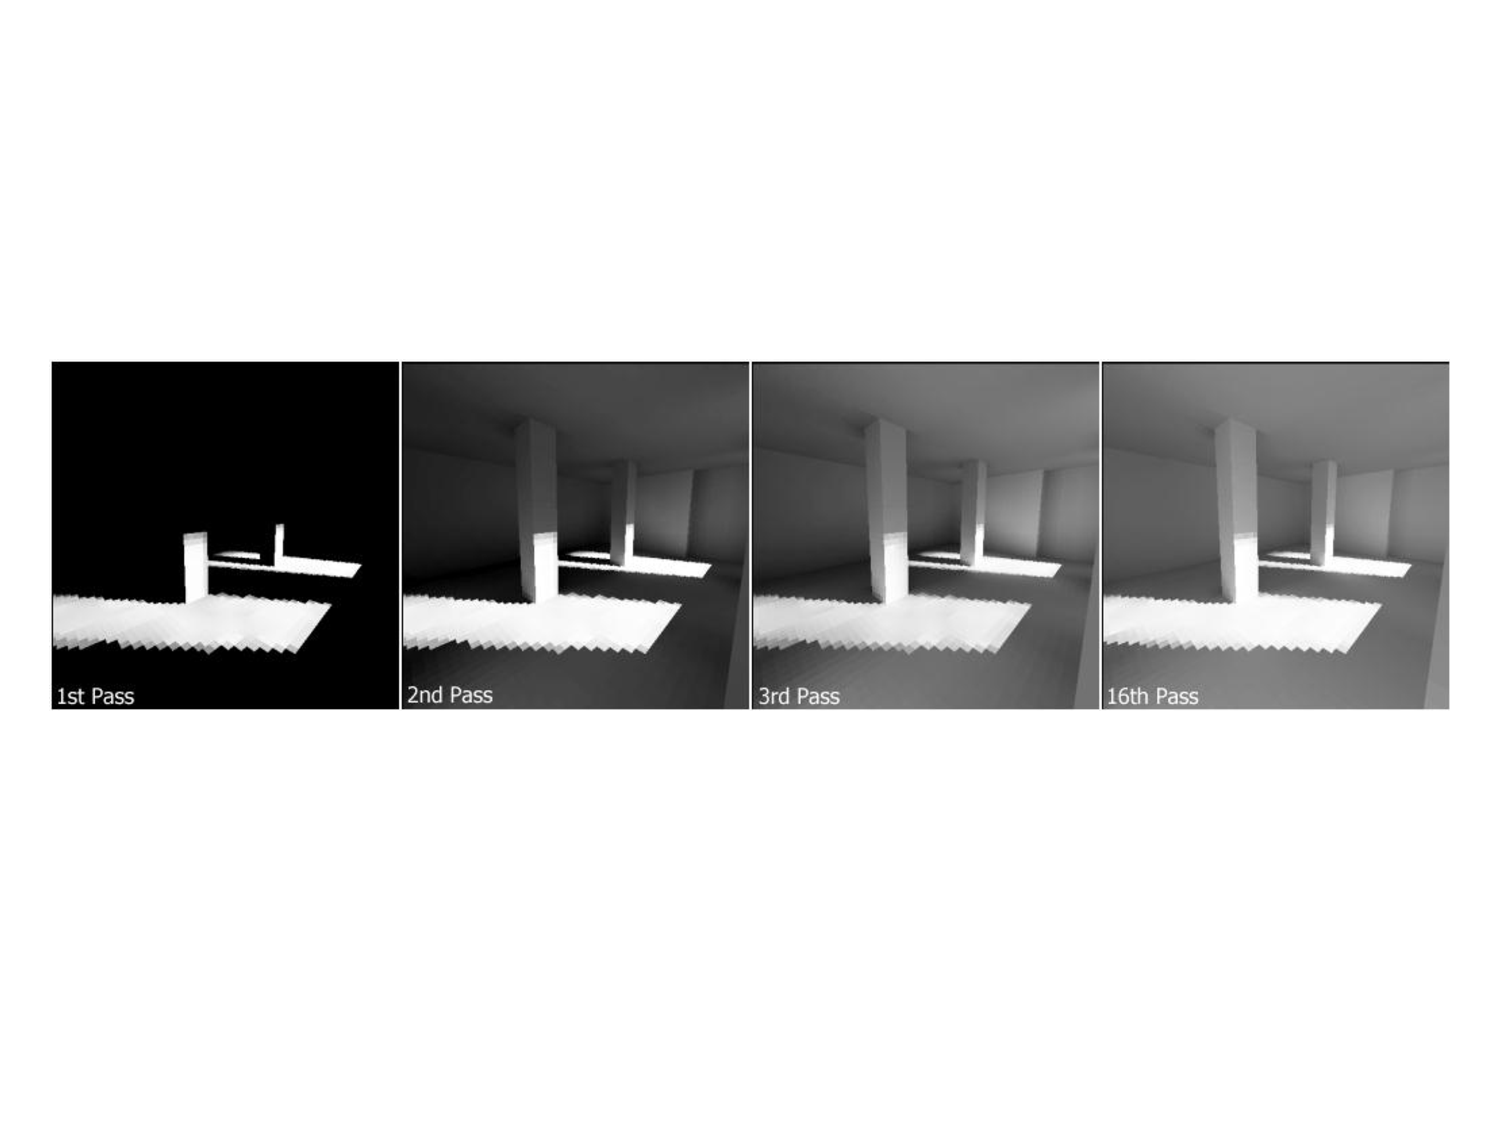
\includegraphics[width=.9\textwidth]{figs/radiosity-iteration.pdf}
    \end{center}
\end{frame}

\begin{frame}{Radiosité : avantages}
    \begin{itemize}
        \item Calcul indépendant du point de vue
        \begin{itemize}
            \item Déplacement interactif (si pas d'impact sur l'environnement)
        \end{itemize}
        \item Adapté aux scènes complexes 
        \begin{itemize}
            \item Sources non ponctuelles 
        \end{itemize}
        \item Partitionnement des échanges lumineux
    \end{itemize}
\end{frame}

\begin{frame}{Radiosité : inconvénients}
    \begin{itemize}
        \item Modèle diffus pur 
        \begin{itemize}
            \item On peut enchaîner sur une phase de ray tracing 
        \end{itemize}
        \item Coût mémoire
        \item Calcul et stockage des facteurs de forme 
        \item Résultats très liés au maillage 
    \end{itemize}
\end{frame}

\begin{frame}{Accélération : radiosité hiérarchique}
    \begin{center}
        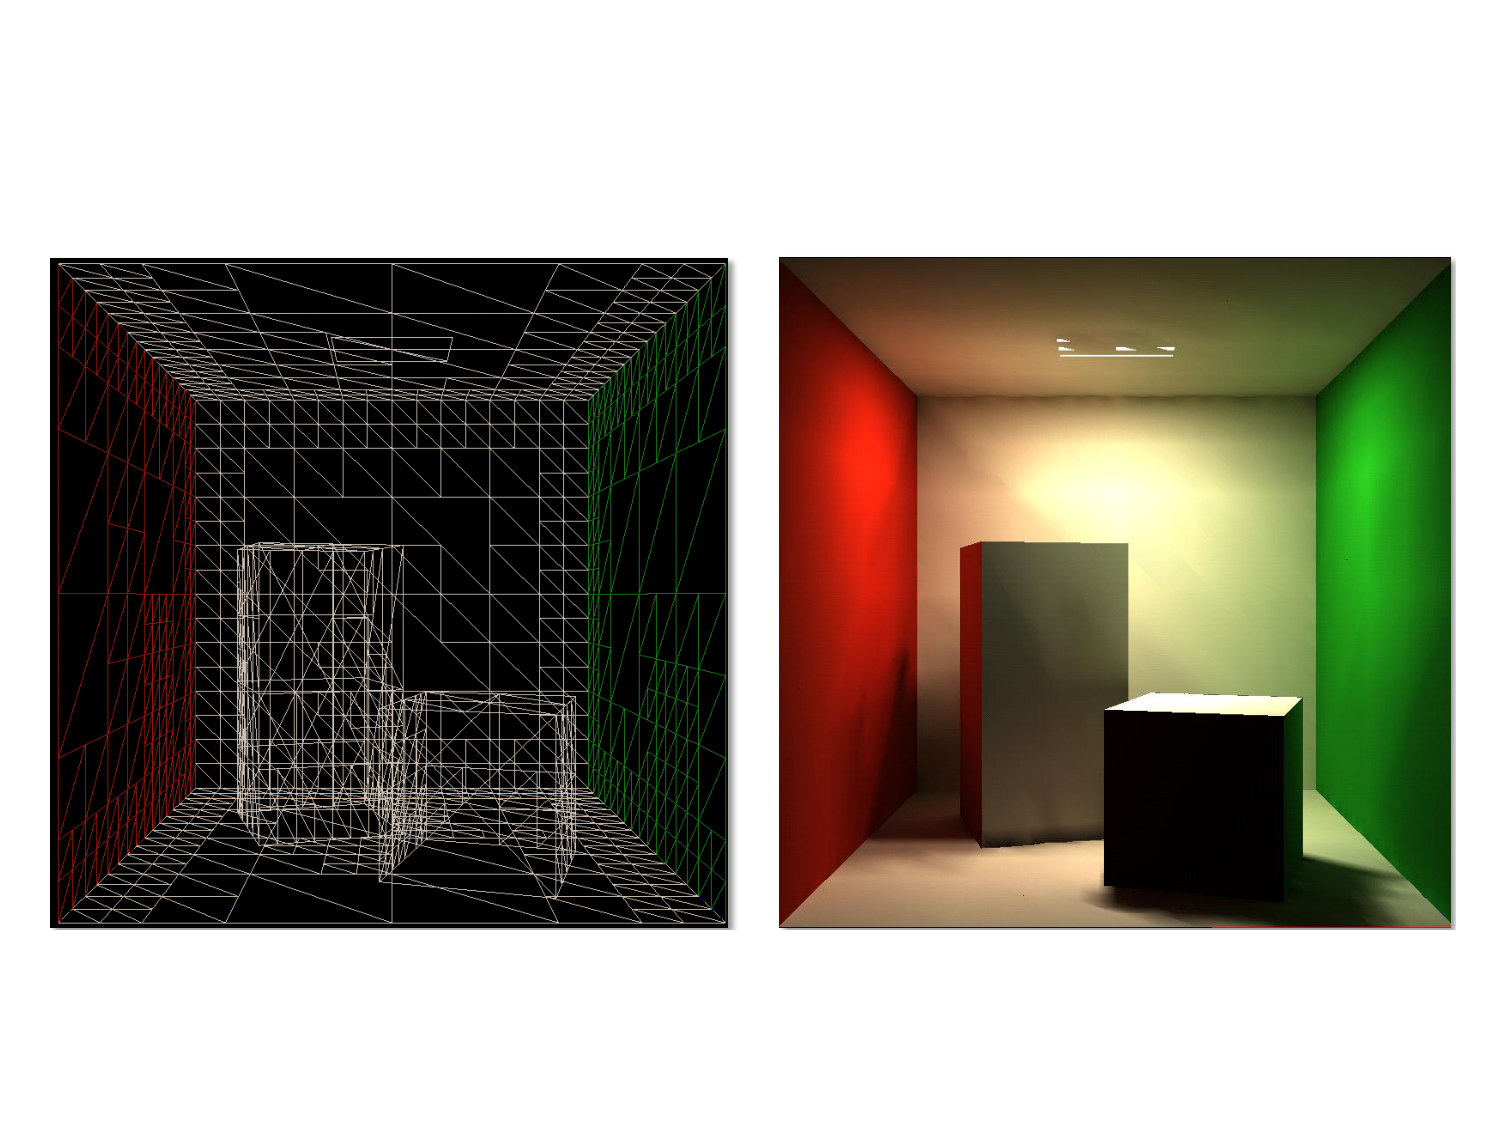
\includegraphics[width=.9\textwidth]{figs/radiosite-hierarchique.pdf}
\end{center}
\end{frame}

\begin{frame}{Améliorations du rendu : maillage des discontinuités}
    \begin{center}
        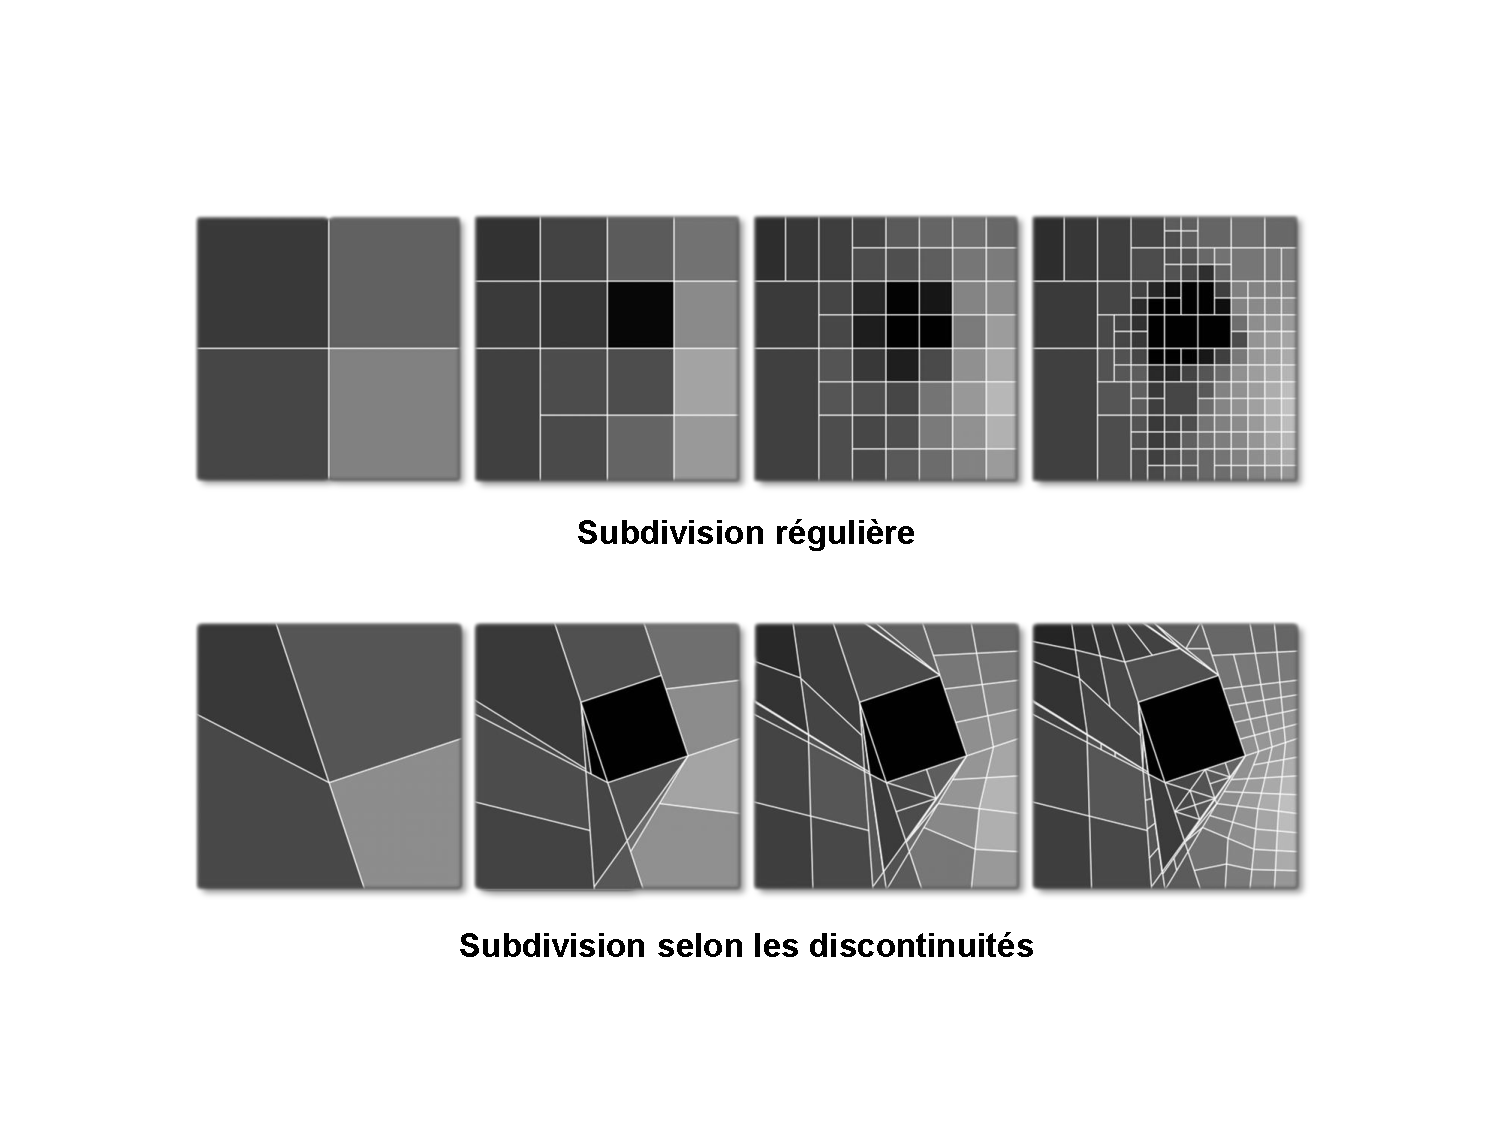
\includegraphics[width=.9\textwidth]{figs/maillage-discontinuite.pdf}
    \end{center}
\end{frame}

\begin{frame}{Maillage des discontinuités : exemple (1/3)}
\begin{center}
    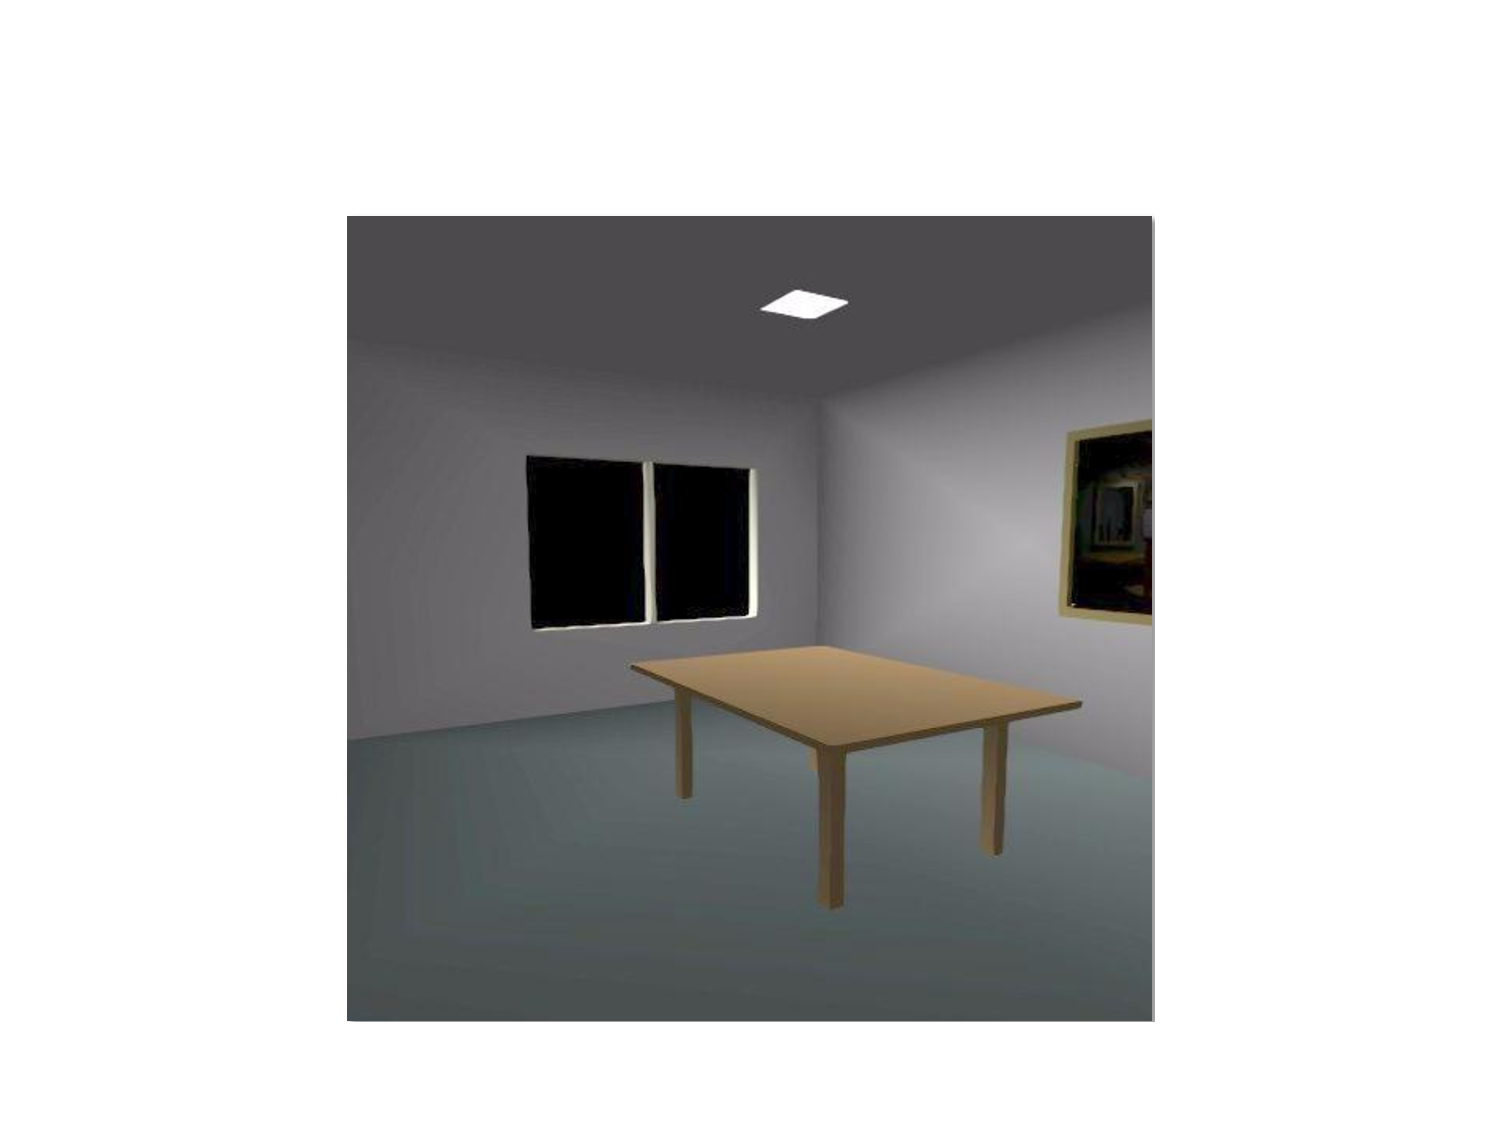
\includegraphics[width=.5\textwidth]{figs/md-1.pdf}
\end{center}    
\end{frame}

\begin{frame}{Maillage des discontinuités : exemple (2/3)}
    \begin{center}
        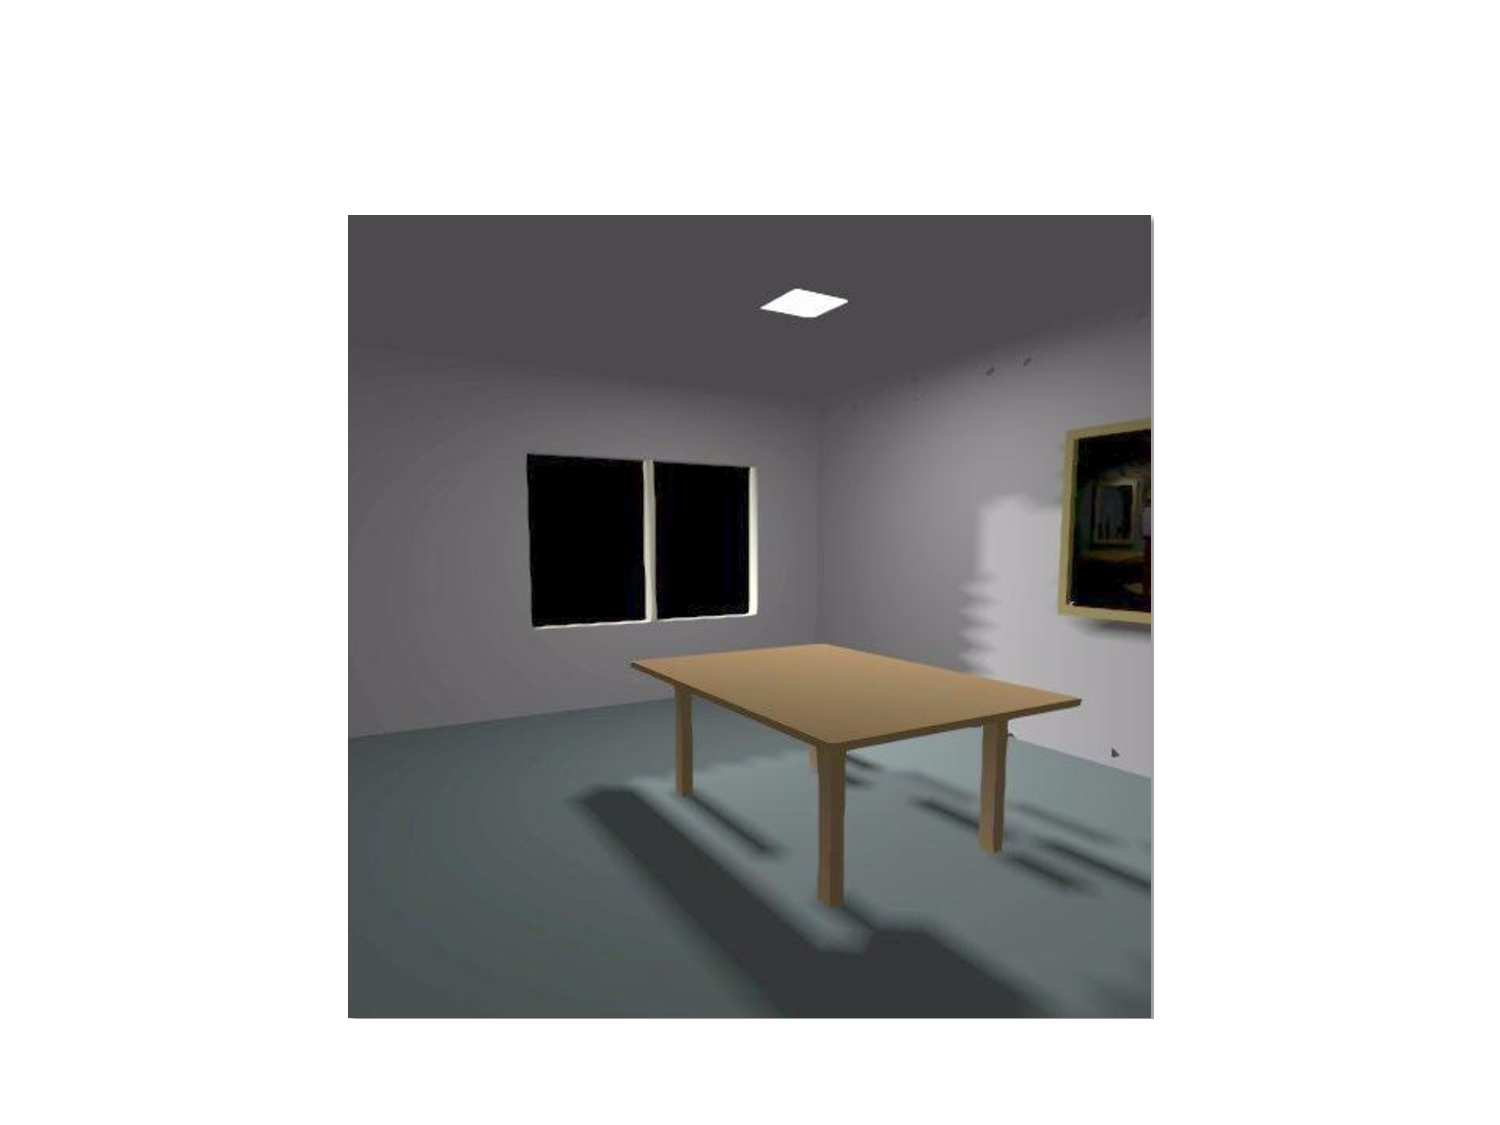
\includegraphics[width=.5\textwidth]{figs/md-2.pdf}
    \end{center}    
    \end{frame}

    \begin{frame}{Maillage des discontinuités : exemple (3/3)}
        \begin{center}
            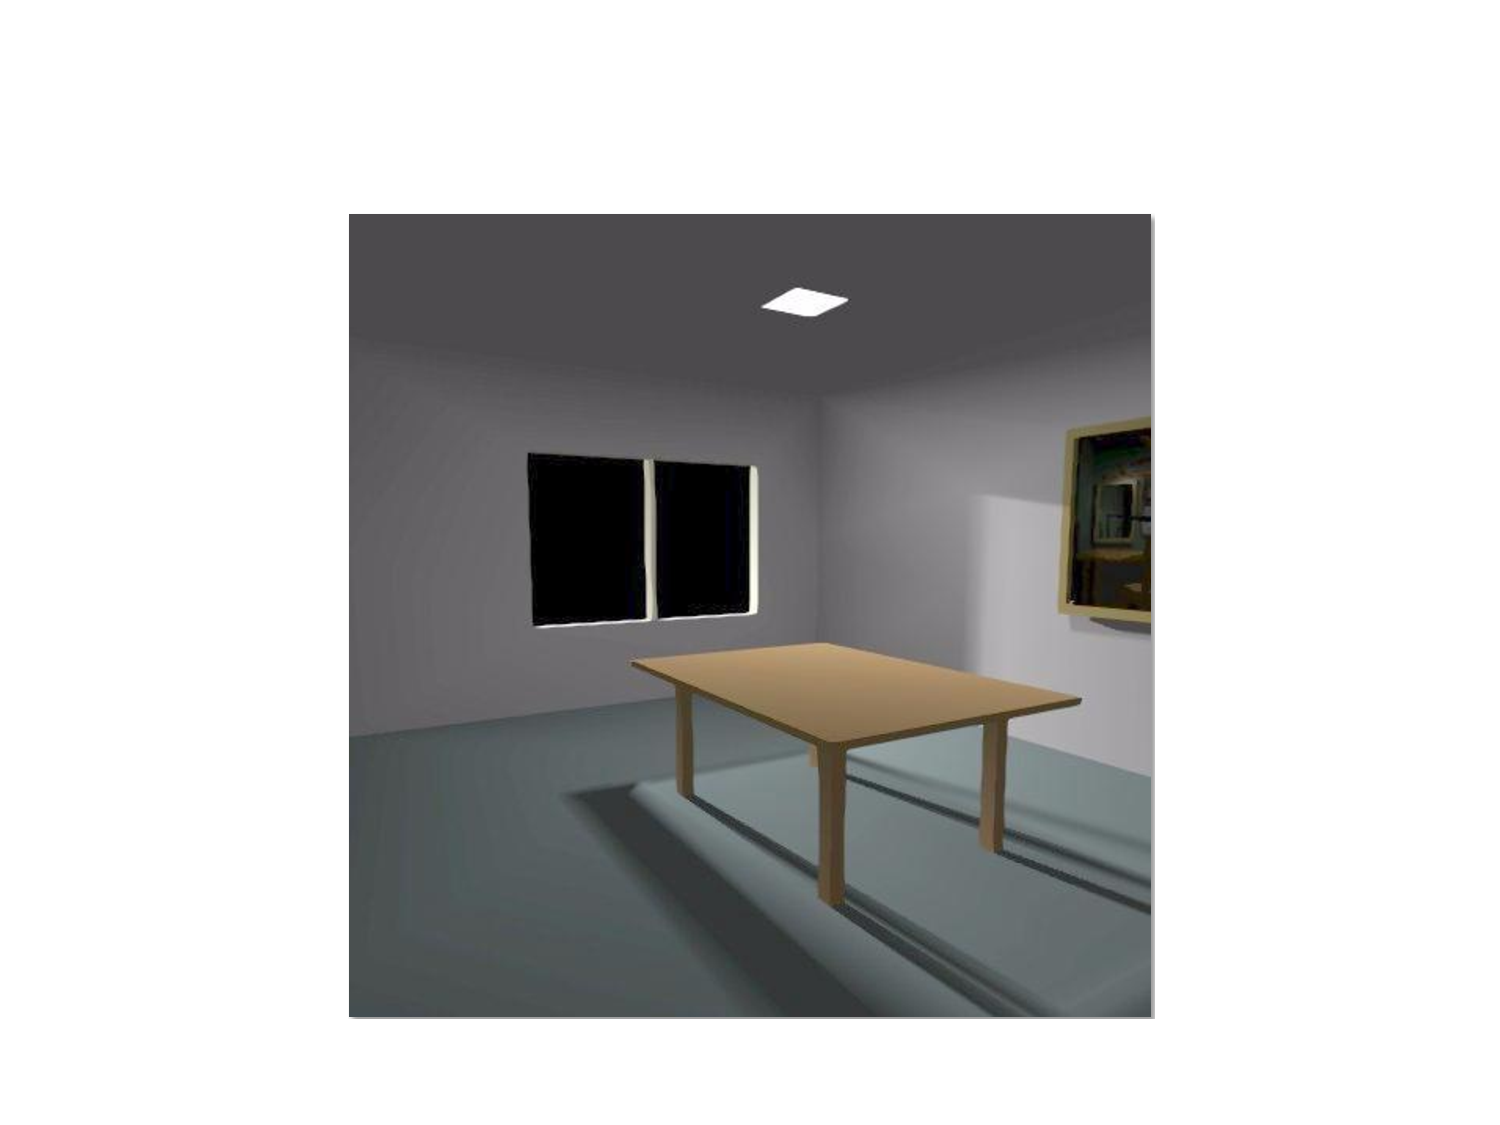
\includegraphics[width=.5\textwidth]{figs/md-3.pdf}
        \end{center}    
        \end{frame}



        